\documentclass[12pt,a4paper]{article}

\usepackage[T1]{fontenc}
\usepackage[utf8]{inputenc}
\usepackage[margin=1in]{geometry}
\usepackage{newtxtext,newtxmath}
\usepackage{microtype}
\usepackage{graphicx}
\usepackage{float}
\usepackage{amsmath,bm}
\usepackage{booktabs}
\usepackage{array}
\usepackage{tabularx}
\usepackage{enumitem}
\usepackage{fancyhdr}
\usepackage{titlesec}
\usepackage{caption}
\usepackage{placeins}
\usepackage[hidelinks,hyperfootnotes=false]{hyperref}
\ifdefined\markedrevision
  \usepackage[switch]{lineno}
\fi

\setlength{\parindent}{1.2em}
\setlength{\parskip}{0.05em}
\linespread{1.05}
\setlist[itemize]{leftmargin=1.2em,itemsep=0.1em,topsep=0.2em}
\setlist[enumerate]{leftmargin=1.35em,itemsep=0.1em,topsep=0.2em}
\emergencystretch=3em

\pagestyle{fancy}
\fancyhf{}
\fancyhead[R]{\thepage}
\setlength{\headheight}{15pt}
\renewcommand{\headrulewidth}{0pt}
\renewcommand{\footrulewidth}{0pt}

\renewcommand{\thesection}{\arabic{section}}
\renewcommand{\thesubsection}{\thesection.\arabic{subsection}}
\renewcommand{\thesubsubsection}{\thesubsection.\arabic{subsubsection}}
\renewcommand{\figurename}{Figure}
\renewcommand{\tablename}{Table}
\captionsetup{font=small,labelfont=bf,labelsep=space}

\titleformat{\section}
  {\large\bfseries}
  {\thesection}
  {0.65em}
  {}
\titleformat{\subsection}
  {\normalsize\bfseries}
  {\thesubsection}
  {0.55em}
  {}
\titleformat{\subsubsection}
  {\normalsize\itshape}
  {\thesubsubsection}
  {0.45em}
  {}
\titlespacing*{\section}{0pt}{1.1em}{0.55em}
\titlespacing*{\subsection}{0pt}{0.85em}{0.3em}
\titlespacing*{\subsubsection}{0pt}{0.75em}{0.25em}

\newcommand{\dd}{\mathrm{d}}
\newcommand{\ii}{\mathrm{i}}
\newcommand{\C}{\mathbb{C}}
\newcommand{\R}{\mathbb{R}}
\begin{document}
\ifdefined\markedrevision
  \color{blue}
  \linenumbers
\fi
\begin{center}
{\Large\bfseries Low-lying quasinormal modes of Kazakov--Solodukhin black holes from Chebyshev and continued-fraction methods}\\
\vspace{1.2em}
{\normalsize Adel H. Al-Yoorby\textsuperscript{1,*}}\\
\vspace{0.25em}
{\itshape \textsuperscript{1}Department of Physics, Khalifa University of Science and Technology,}\\
{\itshape P.O. Box 127788, Abu Dhabi, United Arab Emirates}\\
\vspace{0.25em}
{\small ORCID: 0009-0000-1935-4392}
\end{center}

\begin{center}
\begin{minipage}{0.92\textwidth}
\small
\noindent\textbf{Abstract.}
We investigate how the Kazakov--Solodukhin (KS) deformation changes the
low-lying ringing of a black hole at fixed mass.  The minimally coupled scalar
field provides the cleanest probe.  As the deformation grows, its effective
potential barrier moves outward, becomes lower, and becomes less sharply
curved.  The resulting fundamental modes have a lower oscillation frequency
and a smaller damping magnitude.  For the quadrupolar \(\ell=2,n=0\) mode at
\(a/M=1\), \(\operatorname{Re}\omega\), \(-\operatorname{Im}\omega\), and
\(Q=\operatorname{Re}\omega/[2(-\operatorname{Im}\omega)]\) change by
\(-7.29\%\), \(-2.59\%\), and \(-4.83\%\), respectively.  Thus the scalar
ringing is lower in frequency and lasts slightly longer, but completes fewer
cycles per damping time.  We establish these shifts with Chebyshev collocation
and a collocation-independent Frobenius continued fraction; candidate roots
must pass residual, convergence, continuation, backward-error, and
cross-method checks.  In the Schwarzschild limit, the \(N=96\) scalar result
and the continued-fraction value differ from the published benchmark by
\(5.60\times10^{-11}\) and \(8.24\times10^{-13}\).  We report robust scalar
fundamentals for \(\ell=2,3,4\), cross-validated first overtones at \(N=32\),
and exploratory second overtones.  The scalar pseudospectral basin also
broadens with deformation.  For odd-parity gravitational perturbations we
derive a gauge-invariant master equation under an inverse-Cowling closure;
those axial frequencies remain conditional because the spherical KS action
does not determine nonspherical quantum-source perturbations.

\vspace{0.65em}
\noindent\textbf{Keywords.}
Kazakov-Solodukhin black holes; quasinormal modes; Chebyshev spectral methods; Leaver continued fractions; spectral residual minimization; black-hole spectroscopy.
\end{minipage}
\end{center}
\vspace{1.0em}
\begingroup
\renewcommand{\thefootnote}{*}
\footnotetext{Corresponding author: alyoorby@gmail.com.}
\endgroup
\thispagestyle{empty}

\section{Introduction}

After a black hole is disturbed, it does not vibrate indefinitely.  Part of
the disturbance falls through the horizon and part escapes to infinity,
leaving a short-lived superposition of characteristic ringing modes.  These
quasinormal modes (QNMs) are resonances associated with an effective potential
barrier generated by the spacetime geometry and angular structure.  Their
complex frequencies have an immediate physical meaning:
\(\operatorname{Re}\omega\) sets the pitch of the ringing, while
\(-\operatorname{Im}\omega\) sets the rate at which its amplitude decays.
With the convention \(e^{-i\omega t}\), writing
\(\omega=\omega_R-i\alpha\) gives a damping time
\(\tau=1/\alpha\), where \(\alpha>0\).
The spectrum therefore connects the geometry outside the horizon to black-hole
stability, ringdown, and gravitational-wave tests of compact objects
\cite{Vishveshwara1970,Kokkotas1999,Berti2009,Konoplya2011}.

The first binary-black-hole detection made this regime observationally
accessible \cite{Abbott2016Observation}. Ringdown spectroscopy subsequently
developed into a practical test of the Kerr hypothesis, with both angular
harmonics and overtones entering the analysis \cite{Berti2006,Berti2009,Isi2019}.
Reliable spectra are therefore needed not only for Kerr black holes, but also
for proposed quantum-corrected and exotic geometries whose ringdowns may depart
from the general-relativistic expectation \cite{Konoplya2011,Jaramillo2021}.

QNM frequencies are obtained with several complementary tools.  The
Wentzel--Kramers--Brillouin (WKB) approximation treats the wave locally near
the top of a slowly varying effective-potential barrier and connects the
spectrum to its height and curvature.  It is efficient when the multipole number exceeds
the overtone number \cite{Schutz1985,Iyer1987,Ferrari1984,Konoplya2003,Konoplya2011}. Direct
time-domain evolution extracts the least-damped modes from waveforms, while
Frobenius/Leaver continued fractions impose the frequency-domain boundary
conditions through a minimal-solution recurrence \cite{Leaver1985,Nollert1993}. The
asymptotic iteration method provides another recursive treatment of the radial
ordinary differential equation \cite{Cho2010}.  Spectral and pseudospectral
methods discretize the boundary-value problem globally and often return many
eigenvalues in a single solve \cite{Jansen2017}. Each technique has a different
failure mode: WKB expansions are least reliable for low multipoles and high
overtones, waveform fits favor the least-damped tones, and finite spectral
pencils may contain spurious roots \cite{Konoplya2003,Konoplya2011,Jansen2017}.
We therefore use the Chebyshev spectrum as a starting point and judge each mode
with convergence, continuation, residual, and continued-fraction tests.

The background considered here is the quantum-deformed Schwarzschild metric of
Kazakov and Solodukhin, obtained from a two-dimensional dilaton-gravity
description of spherically symmetric quantum fluctuations \cite{Kazakov1994}.
Its global interpretation requires some care---the deformation improves aspects
of the central geometry without generically satisfying every criterion used for
a regular black hole \cite{Berry2021}---but it provides a well-defined static
metric on which wave propagation can be studied. Earlier calculations found
modest changes in the fundamental QNMs and a much stronger response in parts of
the overtone spectrum \cite{Konoplya2020,Bolokhov2025}.  The central physical
question is consequently simple: at fixed mass, does increasing \(a/M\) make
the exterior potential barrier higher or lower, and how does that change the
pitch and lifetime of the trapped waves?  The Schwarzschild limit supplies the
numerical control experiment; the finite-\(a/M\) branches answer the physical
question.

QNMs are non-self-adjoint resonances, and this matters numerically. Outgoing
boundary conditions lead to complex spectra that may be sensitive to both
operator perturbations and discretization \cite{Jaramillo2021,Cao2024}. We
write the finite Chebyshev problem as \(P_N(\omega)u=0\) and monitor
\(\sigma_{\min}[P_N(\omega)]\). Equivalently,
\(\sigma_{\min}[P_N(\omega)]=
\sqrt{\lambda_{\min}[P_N(\omega)^\dagger P_N(\omega)]}\); the eigenvalue itself
is the square of the singular-value residual. Singular-value tests are standard tools
for nonlinear eigenvalue problems \cite{Sadkane2023}, while related resolvent
and pseudospectral diagnostics have become increasingly important in black-hole
perturbation theory \cite{Jaramillo2021,Cao2024}. Here they are used to decide
whether a root of the generalized Chebyshev pencil is a converged KS resonance.
The Frobenius calculation supplies a numerically distinct, collocation-independent discretization of the
same radial equation and is particularly useful for following a mode as
\(a/M\) changes \cite{Leaver1985,Bolokhov2025}.

Modes are labelled by the spherical-harmonic multipole \(\ell\) and the
overtone index \(n\).  The least-damped mode for a fixed \(\ell\) is the
fundamental, \(n=0\); successively more strongly damped modes are the
overtones \(n=1,2,\ldots\).  Spherical symmetry makes the frequency independent
of the azimuthal label \(m\), which is suppressed.  Here ``low-lying'' means
the fundamental and first few overtones nearest the real-frequency axis.  Our
scope is this low-lying KS spectrum. The
scalar \(n=0\) modes are robust fundamentals; scalar \(n=1\)
branches are cross-validated low-lying first overtones at \(N=32\); \(n=2\) entries are exploratory
branch diagnostics; and higher overtones are outside the scope.  Recent
analytic-continuation methods based on confluent-Heun solutions explicitly
target complete and highly damped spectra of type-D black holes
\cite{Chen2025}; the present calculation is not intended to compete in that
regime. The minimally coupled scalar field gives the cleanest physical probe
of the KS metric because it propagates without perturbing the effective source
that supports the geometry.  The axial, or odd-parity, sector instead
describes metric perturbations with parity \((-1)^{\ell+1}\).  For that sector
we derive the gauge-invariant equation and then impose a frozen-source,
inverse-Cowling closure,
as in perturbative treatments of general spherical backgrounds
\cite{Gerlach1979,Gundlach1999,Karlovini2002}. Those frequencies characterize
the stated effective model, not a unique nonspherical completion of the KS
quantum source.

\subsection{Literature context and related work}

\subsubsection{Quasinormal modes and black-hole spectroscopy}

The theory of black-hole perturbations begins with the Regge--Wheeler analysis of Schwarzschild perturbations \cite{Regge1957} and early numerical recognition of damped black-hole ringing \cite{Vishveshwara1970}. Modern reviews emphasize that QNM spectra provide information about stability, boundary conditions, late-time behavior, and possible observational tests of general relativity \cite{Kokkotas1999,Berti2009,Konoplya2011}. In gravitational-wave astronomy, QNM spectroscopy is especially important because detecting multiple ringdown tones can test whether the remnant is described by the Kerr family \cite{Berti2006,Isi2019}.

\subsubsection{Quantum-corrected Schwarzschild geometries}

Kazakov and Solodukhin proposed a quantum deformation of the Schwarzschild solution in which the radial center is displaced to a Planck-scale surface through a spherically symmetric quantum correction \cite{Kazakov1994}. Later geometric analyses have clarified that the original construction improves some regularity properties but does not automatically remove all curvature singular behavior in the sense usually meant in general relativity \cite{Berry2021}. Phenomenological work on KS black holes has studied QNMs, scattering, shadows, Hawking radiation, and overtone sensitivity \cite{Konoplya2020,Bolokhov2025}. These studies motivate higher-accuracy spectral calculations and systematic comparisons across deformation parameters.

\subsubsection{Spectral approaches to QNM computation}

Spectral methods are attractive for QNM problems because they approximate smooth functions globally and can converge rapidly when the boundary conditions and coordinate compactifications are chosen well. Leaver's Frobenius continued-fraction method remains a standard benchmark for black-hole QNM calculations \cite{Leaver1985}. Jansen's QNM spectral package demonstrates how differential QNM equations can be discretized and solved as generalized eigenvalue problems over a wide class of asymptotics \cite{Jansen2017}. More recent studies by Batic, Dutykh, and collaborators use spectral formulations to revisit noncommutative Schwarzschild black holes, Lee--Wick black holes, and Morris--Thorne wormholes, correcting or sharpening conclusions obtained from lower-order approximation methods \cite{Batic2024Noncomm,Batic2024LeeWick,Batic2024Wormhole}. Pseudospectral and pseudospectrum analyses also highlight that QNM spectra can be sensitive to operator perturbations, an important caution for finite-resolution spectral discretizations \cite{Jaramillo2021}. Cao et al. recently applied this pseudospectrum perspective to a quantum-corrected Schwarzschild black hole, which is especially relevant background for the present KS calculation \cite{Cao2024}.

\subsubsection{Residual and singular-value viewpoints}

For a nonlinear spectral operator \(P(\omega)\), an exact QNM satisfies
\(P(\omega)u=0\) for a nonzero state \(u\). At finite resolution this condition
can be tested through the smallest singular value, while \(P^\dagger P\)
expresses the same defect as a positive-semidefinite Hermitian problem.
Smallest-singular-value methods are well established for nonlinear eigenvalue
problems \cite{Sadkane2023}, and closely related diagnostics occur in
pseudospectral studies of non-self-adjoint black-hole operators
\cite{Jaramillo2021,Cao2024}. We use this viewpoint to refine the KS roots and
then compare them with spectral convergence and a Leaver continued fraction
\cite{Leaver1985,Jansen2017}.

\section{Methods}

\subsection{Kazakov--Solodukhin perturbation problem}

Kazakov and Solodukhin obtained a spherically symmetric quantum deformation of
the Schwarzschild solution by reducing the four-dimensional Einstein theory to
an effective two-dimensional dilaton-gravity problem and choosing a
renormalizable dilaton potential \cite{Kazakov1994}.  We use the areal-radius
form subsequently employed in the KS QNM analysis of Konoplya
\cite{Konoplya2020}:
\begin{equation}
\begin{aligned}
\dd s^2 &=
-f_a(r)\dd t^2 + f_a(r)^{-1}\dd r^2
+ r^2 \dd\Omega^2,\\
f_a(r)&=\frac{\sqrt{r^2-a^2}}{r}-\frac{2M}{r},
\end{aligned}
\label{eq:ksmetric}
\end{equation}
Here \(r\) is the areal radius, \(M>0\) is the mass parameter, and \(a\geq0\)
is a length scale.  The areal radius is defined so that a sphere at coordinate
\(r\) has area \(4\pi r^2\).  The function \(f_a\) is the lapse: it controls
the redshift of static clocks and vanishes at the event horizon.  No radial-coordinate transformation relative to the
convention of Ref.~\cite{Konoplya2020} is made.  In that convention the
present numerical work treats \(a\) directly as the deformation parameter;
no otherwise unused renormalized coupling is introduced.  Reality of the metric coefficients restricts the
coordinate patch to \(r\geq a\).  The outer horizon follows from
\(f_a(r_h)=0\):
\begin{equation}
\sqrt{r_h^2-a^2}=2M,
\qquad
r_h=\sqrt{4M^2+a^2}.
\label{eq:horizonradius}
\end{equation}
Thus \(r_h>a\) for every finite \(a/M\), and the value \(a/M=1\) used below is
not an extremal or degenerate-horizon limit; it is the upper endpoint of the
deformation interval sampled in this study.  Finally,
\(\sqrt{r^2-a^2}/r\to1\) as \(a\to0\), so
\(f_a(r)\to f_0(r)=1-2M/r\) and Eq.~\eqref{eq:ksmetric} reduces directly to
Schwarzschild in standard areal coordinates.

The first perturbation sector is a minimally coupled massless test scalar.
Starting from
\begin{equation}
\Box\Phi=\frac{1}{\sqrt{-g}}\partial_\mu
\left(\sqrt{-g}\,g^{\mu\nu}\partial_\nu\Phi\right)=0
\label{eq:kleingordon}
\end{equation}
and separating variables according to
\begin{equation}
\Phi(t,r,\theta,\phi)=e^{-\ii\omega t}Y_{\ell m}(\theta,\phi)
\frac{\Psi(r)}{r},
\label{eq:scalarseparation}
\end{equation}
with \(\nabla^2_{S^2}Y_{\ell m}=-\ell(\ell+1)Y_{\ell m}\), gives
\begin{equation}
\frac{1}{r^2}\frac{\dd}{\dd r}
\left[r^2 f_a(r)\frac{\dd}{\dd r}\left(\frac{\Psi}{r}\right)\right]
+\left[\frac{\omega^2}{f_a(r)}-\frac{\ell(\ell+1)}{r^2}\right]
\frac{\Psi}{r}=0.
\label{eq:scalarintermediate}
\end{equation}
Introducing the tortoise coordinate \(\dd r_*/\dd r=f_a^{-1}\) reduces this
equation to the Schr\"odinger form.  This coordinate stretches the horizon to
\(r_*\to-\infty\) and spatial infinity to \(r_*\to+\infty\), putting the two
radiative boundaries at the ends of a one-dimensional wave problem:
\begin{equation}
\frac{\dd^2\Psi}{\dd r_*^2}+
\left[\omega^2 - V_{0\ell}(r;a)\right]\Psi=0,
\label{eq:qnmwave}
\end{equation}
where the scalar effective potential is therefore
\begin{equation}
V_{0\ell}(r;a)=f_a(r)\left[\frac{\ell(\ell+1)}{r^2}+\frac{1}{r}\frac{\dd f_a}{\dd r}\right],
\label{eq:scalarpotential}
\end{equation}
in agreement with the minimally coupled scalar equation used in
Ref.~\cite{Konoplya2020}.  QNM boundary conditions select solutions that are
purely ingoing at the horizon and purely outgoing at spatial infinity.  These
conditions mean that energy leaves the exterior region through both ends and
no wave is sent in from either boundary.  They make \(\omega\) complex and the
radial problem non-self-adjoint.

Equation~\eqref{eq:scalarpotential} also gives the useful physical picture.
The \(\ell(\ell+1)/r^2\) term is the angular-momentum barrier, while
\(f_a'/r\) records the radial curvature of the geometry.  Multiplication by
the lapse makes the potential vanish at the horizon and at infinity, leaving a
single barrier outside the hole.  A QNM is a wave concentrated near this
barrier and leaking through both sides.  Moving and lowering the barrier
therefore shifts the oscillation frequency, while changing its width and
curvature changes the leakage rate and hence the damping.

The odd-parity sector requires an assumption beyond the spherical KS
background.  The original KS construction explicitly writes the full metric
as a nonperturbative spherically symmetric part plus small propagating
nonspherical modes and treats the latter classically at leading order
\cite{Kazakov1994}.  Motivated by that separation, we represent the
quantum-corrected spherical background through
\(G_{\mu\nu}=8\pi T^{\mathrm{eff}}_{\mu\nu}\) and set the
\emph{gauge-invariant odd-parity current} of the effective source to zero.
This is an additional inverse-Cowling (frozen-source) closure, not a
constitutive law derived from the spherical KS effective action.  It retains
the KS spherical quantum backreaction but sets the odd part of
\(\delta T^{\mathrm{eff}}_{\mu\nu}\) to zero and therefore neglects
independent nonspherical quantum-source excitations.  The modes below are
conditional on this explicitly defined model.

Physically, this closure lets the odd-parity geometry ring on the
quantum-corrected spherical background while preventing the effective quantum
source itself from carrying an independent odd-parity oscillation.  It is the
gravitational analogue of holding the material source fixed while perturbing
the surrounding field.  Gauge invariance ensures that the master amplitude is
not a coordinate artifact; it does not determine whether the frozen-source
assumption is the unique quantum dynamics.

Here \emph{gauge} refers to the freedom to relabel coordinates without
changing the physical spacetime.  Individual perturbation components can
change under such a relabelling, even though the underlying geometry does not.
A gauge-invariant master variable is a combination in which those coordinate
changes cancel.  It therefore prevents a coordinate artifact from being
mistaken for a physical wave, but it does not determine the dynamics of the
effective quantum source.

To display the gauge invariance, write the background as
\(g_{ab}(y)\dd y^a\dd y^b+r^2(y)\gamma_{AB}\dd z^A\dd z^B\), where
\(a,b\in\{t,r\}\), and expand an odd perturbation as
\begin{equation}
\delta g_{aB}=h_a X_B^{\ell m},
\qquad
\delta g_{AB}=h_2 X_{AB}^{\ell m}.
\label{eq:odddecomposition}
\end{equation}
Under an odd infinitesimal diffeomorphism generated by
\(\xi_A=\Lambda X_A^{\ell m}\),
\begin{equation}
h_a\mapsto h_a-D_a\Lambda+\frac{2D_a r}{r}\Lambda,
\qquad
h_2\mapsto h_2-2\Lambda.
\label{eq:oddgaugetransformation}
\end{equation}
With our harmonic normalization \(h_2=2h\), the one-form
\begin{equation}
k_a=h_a-\frac12 D_a h_2+\frac{D_a r}{r}h_2
\label{eq:oddgaugeinvariant}
\end{equation}
is therefore gauge invariant.  This is Eq.~(18) of
Gundlach and Mart\'inez-Garc\'ia \cite{Gundlach1999}, written in the
Gerlach--Sengupta conventions of Ref.~\cite{Gerlach1979}.  We choose the
two-dimensional volume form so that \(\epsilon^{tr}=+1\) in the static
\((t,r)\) chart and define, as in Eq.~(68) of Ref.~\cite{Gundlach1999},
\begin{equation}
\Pi=\epsilon^{ab}D_b\left(\frac{k_a}{r^2}\right).
\label{eq:axialpi}
\end{equation}
Writing the odd stress perturbation as
\(\delta T_{aB}=\delta t_a^{\mathrm{odd}}X_B\), its gauge-invariant source
one-form is \(L_a=\delta t_a^{\mathrm{odd}}-Q_{\mathrm{bg}}h_a\), where
\(Q_{\mathrm{bg}}\) denotes the coefficient called \(Q\) for the
angular background stress tensor in the notation of
Ref.~\cite{Gundlach1999}; this is their Eq.~(19).  Because it is constructed
from the gauge-invariant matter combination, imposing \(L_a=0\) does not
fix a coordinate gauge.  The general sourced master equation, Eq.~(69) of
Ref.~\cite{Gundlach1999}, is
\begin{equation}
D_a\left[\frac{1}{r^2}D^a(r^4\Pi)\right]
-(\ell-1)(\ell+2)\Pi
=-16\pi\epsilon^{ab}D_bL_a .
\label{eq:sourcedaxial}
\end{equation}
The associated conservation law is
\(D_a(r^2L^a)=(\ell-1)(\ell+2)L\), Eq.~(62) of the same reference.
Our inverse-Cowling closure sets both odd source amplitudes \(L_a=L=0\),
so the conservation equation and the right-hand side of
Eq.~\eqref{eq:sourcedaxial} vanish identically.  Equivalently, Karlovini's
Eqs.~(38), (39), and (46) give
\((D^aD_a-U)\psi=\kappa r\epsilon^{ab}D_a(r^{-2}J_b)\), with the
same source-free reduction \cite{Karlovini2002}.

For the static metric used here, the normalization
\(\Psi_{\mathrm{ax}}=r^3\Pi\) (up to an irrelevant constant) and
\(\dd r_*/\dd r=f_a^{-1}\) remove the first radial derivative from the
source-free equation.  After Fourier decomposition with
\(e^{-\ii\omega t}\), it becomes
\begin{equation}
\frac{\dd^2\Psi_{\mathrm{ax}}}{\dd r_*^2}
+\left[\omega^2-V_{\mathrm{ax},\ell}(r;a)\right]\Psi_{\mathrm{ax}}=0,
\label{eq:axialmaster}
\end{equation}
with the general anisotropic-source potential
\begin{equation}
V_{\mathrm{ax},\ell}
=f_a\left[
\frac{\ell(\ell+1)}{r^2}-\frac{6m(r)}{r^3}
+4\pi\bigl(\rho-p_r\bigr)\right],
\qquad
f_a=1-\frac{2m(r)}{r}.
\label{eq:axialmatterpotential}
\end{equation}
This form is also obtained in the inverse-Cowling treatment of general static
spherical backgrounds [Eqs.~(14)--(17) of Ref.~\cite{Boonserm2013}].

For the KS metric, \(g_{tt}g_{rr}=-1\).  The background Einstein identities
give
\begin{equation}
m(r)=\frac{r}{2}\left(1-f_a\right)
=M+\frac{r-\sqrt{r^2-a^2}}{2},
\quad
4\pi\rho=\frac{m'}{r^2},
\quad
p_r=-\rho.
\label{eq:kseffectivesource}
\end{equation}
Substitution into Eq.~\eqref{eq:axialmatterpotential} yields the
gauge-invariant inverse-Cowling KS axial potential used in all calculations:
\begin{equation}
V_{\mathrm{ax},\ell}(r;a)
=f_a(r)\left[
\frac{\ell(\ell+1)}{r^2}
+\frac{2(f_a-1)}{r^2}
-\frac{f_a'}{r}\right].
\label{eq:reggewheelerpotential}
\end{equation}
At \(a=0\), \(m=M\), \(\rho=p_r=0\), and
Eq.~\eqref{eq:reggewheelerpotential} becomes the Schwarzschild
Regge--Wheeler potential \cite{Regge1957}. For comparison, define the
lapse-substitution potential
\begin{equation}
V_{\mathrm{lapse},\ell}(r;a)
=f_a(r)\left[\frac{\ell(\ell+1)}{r^2}-\frac{6M}{r^3}\right].
\label{eq:lapsecomparison}
\end{equation}
For \(a>0\), the inverse-Cowling potential differs from this comparison
potential by
\begin{equation}
\Delta V_{\mathrm{ax}}
=\frac{f_a}{r^3}\left[
2\!\left(\sqrt{r^2-a^2}-r\right)
-\frac{a^2}{\sqrt{r^2-a^2}}\right],
\label{eq:axialproxycorrection}
\end{equation}
so the two models are not equivalent.  The same
effective-source potential is also used in the public high-precision
Chebyshev calculation of Batic, Dutykh, and Sukaiti
\cite{BaticDutykhSukaiti2026}; Section~3 compares overlapping modes directly.
We use this potential to compute the low-lying spectrum with two numerically
distinct radial discretizations, monitoring residuals, backward error, continuation in
\(a/M\), and local pseudospectral sensitivity. Gauge
invariance removes coordinate artifacts from the metric master variable; it
does not make the inverse-Cowling closure unique.  A nonspherical quantum-source
action could instead generate a nonzero right-hand side or additional
couplings in Eq.~\eqref{eq:sourcedaxial} \cite{Gerlach1979,Gundlach1999,Karlovini2002}.

\subsection{Numerical method}

We determine the same physical resonances using two numerically distinct
frequency-domain representations.  The Chebyshev calculation describes the radial wave globally
on a compact grid and produces candidate ringing frequencies.  The Frobenius
calculation instead expands the wave locally and enforces the horizon and
infinity conditions through a continued fraction.  Agreement between them
shows that a reported mode is tied to the wave equation and its radiative
boundaries rather than to one discretization.  A time-domain evolution of the
scalar equation provides an additional, lower-precision check on the direction
and scale of the frequency shift, following earlier KS studies
\cite{Konoplya2020}.  The quantitative spectrum comes from the two
frequency-domain calculations \cite{Leaver1985,Jansen2017}; the matrix-pencil
fit to the waveform is only an orientation diagnostic.

\subsubsection{Baseline time-domain diagnostic}

The \emph{time domain} means solving directly for the waveform as a function
of time and then fitting its ringdown.  It answers the intuitive question
``what would the decaying signal look like after an initial pulse?''  This
method is especially good at recovering the least-damped mode because that
mode survives longest, but several damped sinusoids can be difficult to
separate in a short or noisy time interval.  We therefore use it to check the
sign and approximate size of the deformation shift, not to set the final
digits.

The baseline evolves the radial wave equation in tortoise coordinate \(x=r_*\),
\begin{equation}
\frac{\partial^2\Psi}{\partial t^2}
-
\frac{\partial^2\Psi}{\partial x^2}
+
V_{0\ell}(r(x);a)\Psi=0.
\label{eq:timedomain}
\end{equation}
For orientation, Eq.~\eqref{eq:timedomain} is evolved on
\(x/M\in[-250,500]\), with \(\Delta x=0.1M\), \(\Delta t=0.05M\),
\(t_{\max}=320M\), and observation point \(x_{\mathrm{obs}}=20M\). A Gaussian
pulse \(\Psi(0,x)=\exp[-(x/4M)^2]\) is evolved with first-order outgoing
boundary conditions, as in standard time-domain QNM extractions
\cite{Gundlach1994,Konoplya2011,Konoplya2020}. The interval \(60M\leq t\leq160M\) is fitted by
\begin{equation*}
\Psi_{\mathrm{fit}}(t)=A e^{-\alpha(t-t_0)}
\cos(\omega_R t+\phi)+C_0,
\qquad
\omega_{\mathrm{fit}}=\omega_R-\ii\alpha.
\end{equation*}
A rank-four matrix-pencil reduction is also applied to the same waveform
\cite{Hua1990}. It
recovers the expected ringdown scale and deformation trend, but no frequency
reported as a spectral result is inferred from this fit.
Here a \emph{matrix pencil} is a signal-processing construction that represents
the sampled waveform as a sum of damped exponentials; its eigenvalues encode
their frequencies and decay rates.  It should not be confused with the
generalized matrix pencil obtained below from the differential equation.

\subsubsection{Chebyshev spectral discretization}

Chebyshev polynomials are oscillatory global functions on \([-1,1]\) whose
special nodes are dense near the endpoints.  Interpolating at these nodes
reduces large endpoint errors and gives differentiation matrices that
differentiate the interpolating polynomial.  \emph{Collocation} means that we
require the differential equation to hold at each node.  Increasing \(N\)
raises the polynomial resolution and supplies a direct convergence test.

The direct spectral method compactifies the horizon-to-infinity domain with
\begin{equation*}
s=1-\frac{r_h}{r},\qquad x=2s-1,\qquad x\in[-1,1],
\end{equation*}
where \(r_h=\sqrt{4M^2+a^2}\). Chebyshev-Gauss collocation points
\begin{equation*}
x_j=\cos\left(\frac{\pi(j+1/2)}{N}\right),\qquad j=0,\ldots,N-1,
\end{equation*}
are mapped to \(s_j=(x_j+1)/2\), excluding the two singular endpoints.
Barycentric differentiation matrices \(D\) and \(D^2\) approximate
\(\partial_s\) and \(\partial_s^2\), following the usual pseudospectral
treatment of QNM boundary-value problems \cite{Jansen2017}.

The QNM boundary behavior is imposed analytically by factoring
\begin{equation}
\Psi(r)=
e^{\ii\omega r}\,
r^{2\ii M\omega}\,
s^{-\ii\omega/f_a'(r_h)}\,u(s).
\label{eq:factoredfield}
\end{equation}
The factorization in Eq.~\eqref{eq:factoredfield} builds the outgoing behavior
at infinity and the ingoing behavior at the horizon into the unknown, leaving
\(u(s)\) regular on the collocation grid \cite{Leaver1985,Jansen2017}.
Substitution into Eq.~\eqref{eq:qnmwave} gives the quadratic eigenvalue problem
\begin{equation}
P_N(\omega)\bm{u}
\equiv
\left(A_0+\omega A_1+\omega^2A_2\right)\bm{u}=0.
\label{eq:polynomialproblem}
\end{equation}
The matrices \(A_0,A_1,A_2\) are built directly from \(f_a(r)\), \(f_a'(r)\), the selected potential \(V_{0\ell}\) or \(V_{\mathrm{ax},\ell}\), and the chain-rule factors relating \(r\) and \(s\).

\subsubsection{Residual test and mode selection}

The eigensolver is deliberately treated as a candidate generator.  The reason
is that an algebraic eigenvalue of a finite matrix need not approximate a QNM
of the original differential equation.  The residual asks whether some
normalized discrete wavefunction actually satisfies that equation at the
trial frequency.  A singular value is a non-negative measure of how strongly
a matrix stretches vectors; \(\sigma_{\min}\) is the weakest stretching
direction.  It vanishes exactly when the matrix has a nonzero null vector.

For a trial frequency we evaluate the residual map
\begin{equation*}
\omega \mapsto \sigma_{\min}\!\left(P_N(\omega)\right),
\end{equation*}
where \(P_N(\omega)\) is the finite-dimensional Chebyshev representation of
the factored radial equation. A true finite-dimensional eigenfrequency drives
this singular value to zero; in floating-point arithmetic a well-resolved mode
appears as a sharp local minimum. This is the same singular-value viewpoint
used in nonlinear eigenvalue analysis and black-hole pseudospectra
\cite{Sadkane2023,Jaramillo2021,Cao2024}.

The quadratic pencil first supplies possible roots in a damped frequency
window. We then minimize \(\sigma_{\min}[P_N(\omega)]\) locally, compare the
mode across several values of \(N\), follow it continuously in \(a/M\), and
solve the corresponding Frobenius recurrence. The tables report the frequency
together with the raw residual, a scale-aware polynomial backward error, and
the branch classification. In this way the generalized eigensolve locates the
resonance, while convergence and the continued fraction determine how much
confidence can be attached to it \cite{Leaver1985,Jansen2017}.

\subsubsection{Generalized eigenproblem and residual}

The equation is \emph{quadratic} because it contains \(1\), \(\omega\), and
\(\omega^2\).  Linearization doubles the state vector and rewrites it as a
\emph{generalized eigenproblem} \(Az=\omega Bz\).  The pair \((A,B)\) is often
called a matrix pencil.  Its generalized eigenvalues are easy to compute, but
the doubling and the different coefficient scales can amplify roundoff; this
is why the resulting frequencies are candidates rather than accepted modes.

Equation~\eqref{eq:polynomialproblem} is linearized as
\begin{equation}
\begin{pmatrix}
0&I\\
-A_0&-A_1
\end{pmatrix}
\begin{pmatrix}
\bm{u}\\
\omega\bm{u}
\end{pmatrix}
=
\omega
\begin{pmatrix}
I&0\\
0&A_2
\end{pmatrix}
\begin{pmatrix}
\bm{u}\\
\omega\bm{u}
\end{pmatrix},
\label{eq:linearizedspectral}
\end{equation}
We solve Eq.~\eqref{eq:linearizedspectral} with
\(\texttt{scipy.linalg.eig}\). Its roots are initial guesses rather than final
frequencies, since polynomial linearizations can magnify scaling and
conditioning problems. The scalar \(\ell=2\) fundamental is identified from
the Schwarzschild spectrum, whereas overtones are followed by continuity of
both frequency and eigenfunction and are checked separately with the
continued fraction \cite{Leaver1985,Jansen2017}.

\subsubsection{Root filtering, refinement, and branch assignment}

\emph{Equilibration} rescales rows and columns so that very large and very
small coefficients enter the eigensolve on comparable numerical scales.  In
exact arithmetic this does not change a finite eigenvalue; in floating-point
arithmetic it can reduce avoidable loss of precision.  Filtering then removes
frequencies outside the damped physical window and merges duplicate numerical
representatives.  Refinement varies the real and imaginary parts of \(\omega\)
to find the bottom of the local residual basin.  Branch assignment is a
separate step: it asks which refined root is the continuation of a particular
\((\ell,n)\) mode rather than merely which root is closest at one parameter
value.

The selection rules are fixed before the spectrum is computed. Before solving
the pencil, each row of the pair of
linearized matrices is divided by the larger of its two row infinity norms;
the same operation is then applied columnwise after row scaling.  Scaling
factors are clipped to \([10^{-100},10^{100}]\), and the right generalized
eigenvectors are mapped back to the unscaled coordinates.  Infinite and
non-finite roots are removed.  The physical search window is
\(0.05<\operatorname{Re}\omega<2\) and
\(-3<\operatorname{Im}\omega<-0.02\).  Roots separated by at most
\(10^{-7}\) are treated as one numerical cluster, retaining the representative
with the smaller raw-polynomial singular-value residual.  At most the 20
candidates closest to the current branch target enter the detailed scoring stage.

For a previously tracked branch, a candidate must lie within an absolute
complex-frequency distance \(0.20\) of the preceding target.  Competing
matches minimize

\begin{equation*}
S=d_{\rm target}+0.45d_{\rm cont}+0.35(1-|\langle u_{j-1},u_j\rangle|)
+10^{-3}\min(\sigma_j/\sigma_{\rm best},100),
\end{equation*}
where, for the shortlisted candidate set \(\mathcal C\),
\begin{equation*}
d_{\rm target}=\frac{|\omega_j-\omega_{\rm target}|}
{\max(|\omega_{\rm target}|,0.1)},\qquad
d_{\rm cont}=\frac{|\omega_j-\omega_{j-1}|}
{\max(|\omega_{j-1}|,0.1)},\qquad
\sigma_{\rm best}=\min_{k\in\mathcal C}\sigma_k.
\end{equation*}
Here \(\sigma_j=\sigma_{\min}[P_N(\omega_j)]\) is evaluated on the raw,
unequilibrated polynomial matrices at the unrefined generalized-eigenvalue
candidate.  Candidate frequencies and right eigenvectors are generated from
the row- and column-equilibrated linearized pencil; before overlap evaluation,
the right eigenvectors are mapped back by the column-scaling matrix as
\(x=D_r y\).  The extracted mode shapes are normalized, and the previous shape
is barycentrically interpolated to the new grid.  The absolute value in
\(|\langle u_{j-1},u_j\rangle|\) removes the arbitrary complex phase of either
eigenvector.
The selected raw root is refined within a rectangular radius \(0.02\) in each
complex-frequency component by L-BFGS-B minimization of
\(\sigma_{\min}^2[P_N(\omega)]\), with at most 500 iterations,
\texttt{ftol}\(=10^{-18}\), and \texttt{gtol}\(=10^{-12}\).

The catalogue labels \(n=0,1,2\) begin from the stated Schwarzschild seeds;
after each deformation value, the corresponding continued-fraction roots
become the three targets for the next value, and already assigned roots are
excluded within \(10^{-7}\). A catalogue row is retained only when its
raw-polynomial backward error is below \(10^{-8}\) and its
spectral--continued-fraction relative difference is below \(10^{-4}\). These
thresholds remove clearly unresolved roots, but they do not by themselves
establish the physical reliability of a branch. In particular, the \(n=2\)
modes remain exploratory because their convergence is visibly less uniform.

For completeness, the implemented sequence is: (1) equilibrate and solve the quadratic
pencil; (2) remove non-finite roots and roots outside the damped window;
(3) cluster at \(10^{-7}\); (4) enforce the \(0.20\) continuation gate and
score competing matches; (5) refine the selected Chebyshev root by bounded
singular-value minimization; (6) apply the backward-error and
spectral--continued-fraction gates; and (7) propagate the accepted
continued-fraction root as the next deformation target.  Thus the
continued-fraction calculation is collocation-independent, although it shares
the perturbation equation and endpoint factorization.

The direct spectral residual is
\begin{equation}
R_N(\omega)=P_N(\omega)^\dagger P_N(\omega).
\label{eq:directresidual}
\end{equation}
Equation~\eqref{eq:directresidual} is Hermitian and positive semidefinite up to
roundoff. We quote \(\sigma_{\min}[P_N(\omega)]\) and the scale-aware polynomial
backward error, but neither number is meaningful in isolation: a small residual
can accompany a poorly conditioned or nonconvergent discretized root
\cite{Sadkane2023}. Spectral-size convergence and the continued-fraction result
therefore carry equal weight in the mode assignment.

\subsubsection{Leaver-style validation}

As a collocation-independent frequency-domain calculation, we also solve a Frobenius
recurrence in the manner of Leaver \cite{Leaver1985,Nollert1993}.  A Frobenius
series is a power series multiplied by the known singular behavior at an
endpoint.  Substitution converts the differential equation into a recurrence
among series coefficients.  For a generic frequency the recurrence contains a
solution that grows and violates the required boundary behavior; the continued
fraction is the condition that selects the minimal, physically admissible
coefficient sequence.  It uses the same compact
coordinate \(s=1-r_h/r\) and the same physical endpoint behavior, but no
Chebyshev grid, matrix-pencil roots, or singular-value minimization. We write
\begin{equation*}
\Psi(r)=e^{\ii\omega r}r^{2\ii M\omega}s^{-\ii\omega/f'(r_h)}u(s),
\end{equation*}
and expand the regular factor as a Frobenius series,
\begin{equation*}
u(s)=\sum_{n=0}^{\infty} a_n s^n.
\end{equation*}
Substitution into the factored radial equation gives
\begin{equation*}
B_2(s)u''+B_1(s)u'+B_0(s)u=0,
\end{equation*}
where the \(B_j(s)\) are generated by formal power-series algebra from the KS metric functions. The Taylor-truncated Frobenius equations define a multi-term recurrence for the coefficients \(a_n\). Gaussian elimination reduces this recurrence to the three-term form
\begin{equation*}
\alpha_n a_{n+1}+\beta_n a_n+\gamma_n a_{n-1}=0,
\end{equation*}
and the minimal-solution condition is imposed through Leaver's continued fraction,
\begin{equation}
\beta_0-\frac{\alpha_0\gamma_1}{\beta_1-\dfrac{\alpha_1\gamma_2}{\beta_2-\cdots}}=0.
\label{eq:leaver}
\end{equation}
The reported calculation expands each \(B_j\) through Taylor order 96 and
evaluates the reduced recurrence to continued-fraction depth 240.  Roots of
Eq.~\eqref{eq:leaver} are obtained in IEEE-754 double precision by applying the
MINPACK hybrid solver exposed by \texttt{scipy.optimize.root} to the real and
imaginary residual components.  The root tolerance is \(10^{-11}\), the maximum
number of residual-function evaluations is 1000, and the accepted residual is
required to be below \(10^{-7}\) for the scalar validation calculation.  The
initial guesses are the branch-tracked \(N=32\) Chebyshev candidates. At
\(a/M=0\), those candidates are selected as the nearest distinct roots to the
18 literature targets listed in Table~\ref{tab:schwarzschildseeds} of
Appendix~\ref{sec:schwarzschildseeds}; no
manual or continued-fraction Schwarzschild seed is used. Branch
identity is maintained by continuation over \(a/M=0,0.2,0.5,1\) and by keeping
the fundamental and first-overtone targets distinct.  The catalogue uses the
same settings, with a relaxed \(10^{-4}\) residual acceptance threshold for the
most delicate second-overtone recurrence reductions. This validation layer is
collocation-independent: it uses no Chebyshev grid, matrix-pencil data, or residual
minimization, while sharing the same perturbation equation and endpoint
factorization.

\section{Results}

Before discussing numerical accuracy, it is useful to state the physical
effect visible in the scalar wave equation.  At fixed \(M\), increasing the
deformation from \(a/M=0\) to \(1\) moves the horizon from \(r_h/M=2\) to
\(\sqrt{5}\).  For the \(\ell=2\) scalar barrier, the peak moves from
\(r/M=2.9517\) to \(3.2520\), its height falls by \(13.54\%\), and the
magnitude of its tortoise-coordinate curvature falls by \(17.77\%\).  The
leading WKB estimate \(\operatorname{Re}\omega\sim\sqrt{V_{\rm peak}}\)
therefore predicts a \(7.01\%\) decrease in oscillation frequency, close to
the fully computed \(7.29\%\) shift.  The damping rate depends on both the
barrier curvature and the global outgoing-wave solution, so it need not fall
by the same fraction; the numerical mode gives a smaller \(2.59\%\) decrease
in damping magnitude.

In time-domain language, the deformed scalar signal would have a lower pitch
and a slightly more slowly decaying envelope.  Because the pitch falls more
than the damping rate, the signal nevertheless completes fewer oscillations
within one damping time: its quality factor decreases by \(4.83\%\).  The
\(\ell=3\) and \(4\) barriers show the same behavior, so this is a systematic
low-lying scalar effect rather than an isolated quadrupole feature.  The
following validation establishes that these percent-level changes are much
larger than the numerical uncertainty.

\subsection{Schwarzschild validation}

As an external benchmark we use the spin-zero Schwarzschild fundamental with
\(\ell=2\), overtone index \(n=0\), mass normalization \(M=1\), time dependence
\(e^{-\ii\omega t}\), and therefore \(\operatorname{Im}\omega<0\) for a damped
mode.  In the neutral Schwarzschild limit \(q=Q=0\), Cavalcante and da Cunha
report the spin-zero \(\ell=2\) entry in Table~I on page~6 from an
isomonodromic Painlev\'e calculation and reproduce it in the adjacent column
with a continued-fraction method \cite{Cavalcante2021}.  After matching our
\(e^{-\ii\omega t}\) convention, the value is
\begin{equation*}
M\omega_{\mathrm{ref}}=0.483643872211-0.096758775978\,\ii.
\end{equation*}
Throughout the numerical comparisons we use
\begin{equation*}
\Delta_{\mathrm{rel}}(\omega_1,\omega_2)
=\frac{|\omega_1-\omega_2|}{|\omega_2|}.
\end{equation*}
Here \(\omega_2\) is the reference value.
At \(N=96\), the direct spectral calculation gives
\begin{equation*}
M\omega_{\mathrm{spec}}=0.483643872189-0.096758775961\,\ii,
\end{equation*}
with relative difference \(5.60\times10^{-11}\) from that external value. This is substantially sharper than the baseline time-domain fit, \(0.483642480-0.096758919\,\ii\), and the waveform matrix-pencil diagnostic, \(0.483653530-0.096763421\,\ii\).

The Leaver-style solver gives
\begin{equation*}
M\omega_{\mathrm{Leaver}}=0.483643872211-0.096758775978\,\ii
\end{equation*}
for the Schwarzschild fundamental mode, with relative difference
\(8.24\times10^{-13}\) from the same external value. Such accuracy is routine
for mature Schwarzschild solvers \cite{Leaver1985,Cavalcante2021}; its role here
is to verify the conventions, endpoint factors, and branch identification in
both of our frequency-domain implementations.

Figure~\ref{fig:spectralconvergence} shows how the Chebyshev roots approach an
order-128, depth-320 continued-fraction value. The fundamental settles onto a
double-precision plateau. The first overtone behaves differently: agreement is
best near \(N=32\)--48 and worsens as the differentiation matrices become more
ill-conditioned at larger \(N\), a familiar limitation of high-order
collocation in finite precision \cite{Jansen2017}. We therefore describe these
modes as cross-validated low-lying first overtones at \(N=32\), rather than
interpreting the largest available grid as automatically the most accurate.

\begin{figure}[H]
\centering
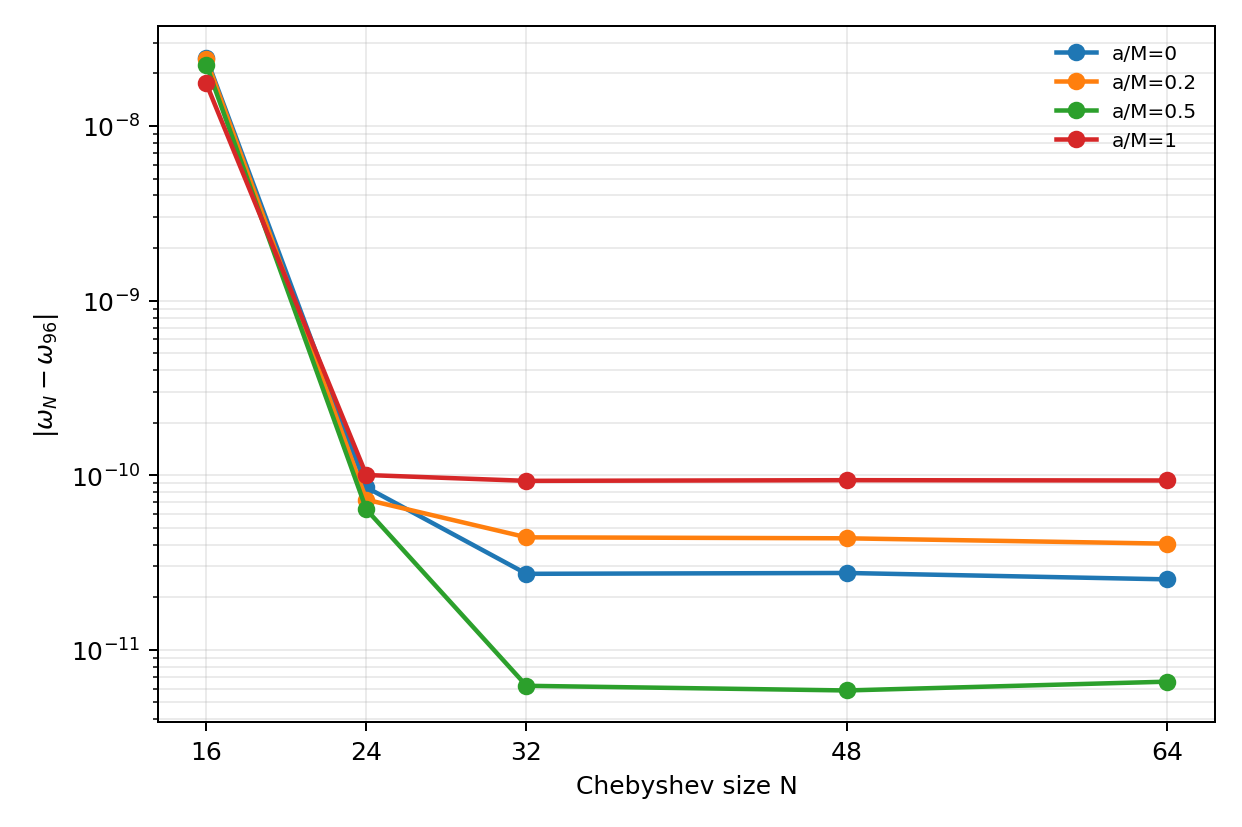
\includegraphics[width=\linewidth]{figures/figure1_spectral_convergence.png}
\caption{Chebyshev error relative to the order-128, depth-320 continued-fraction root for scalar \(\ell=2\) fundamentals (left) and first overtones (right), including \(N=128\). The overtone panel displays the high-\(N\) deterioration directly.}
\label{fig:spectralconvergence}
\end{figure}

As an upper-grid check, we also recomputed the scalar \(\ell=2,n=0\) branch at
\(N=128\) for \(a/M=0\) and \(1\). The shifts from \(N=96\) are
\(6.95\times10^{-11}\) and \(4.64\times10^{-10}\), respectively, far below
the scale of any deformation trend reported below. The small nonmonotonic motion
between \(N=96\) and \(128\) is consistent with roundoff amplification in the
differentiation matrices and the linearized pencil \cite{Jansen2017}. We use
\(N=96\) for the fundamental catalogue and take the collocation-independent
continued fraction as the external numerical anchor.

\subsection{Leaver continued-fraction comparison}

Table~\ref{tab:leavercomparison} summarizes the Leaver-style continued-fraction validation against the targeted Chebyshev spectral rows used for the scalar comparison.

\begin{table}[H]
\centering
\footnotesize
\renewcommand{\arraystretch}{1.14}
\begin{tabular}{llrrr}
\toprule
\(a/M\) & mode &
\(\mathrm{Re}(M\omega_{\mathrm{Leaver}})\) &
\(\mathrm{Im}(M\omega_{\mathrm{Leaver}})\) &
\(\Delta_{\mathrm{rel}}(\mathrm{spec},\mathrm{Leaver})\)\\
\midrule
0.0 & fundamental & 0.48364387 & -0.09675878 & \(7.914\times10^{-13}\)\\
0.0 & first overtone & 0.46385058 & -0.29560394 & \(1.814\times10^{-9}\)\\
0.2 & fundamental & 0.48203369 & -0.09665386 & \(6.084\times10^{-13}\)\\
0.2 & first overtone & 0.46216559 & -0.29531130 & \(1.788\times10^{-9}\)\\
0.5 & fundamental & 0.47388693 & -0.09610918 & \(6.219\times10^{-13}\)\\
0.5 & first overtone & 0.45364275 & -0.29379018 & \(1.808\times10^{-9}\)\\
1.0 & fundamental & 0.44836241 & -0.09424818 & \(6.341\times10^{-13}\)\\
1.0 & first overtone & 0.42697149 & -0.28857291 & \(1.747\times10^{-9}\)\\
\bottomrule
\end{tabular}
\caption{Leaver-style continued-fraction validation against targeted Chebyshev spectral results at \(N=32\). Frequency columns are rounded for display; the discrepancy column is computed from full-precision internal values. The Leaver solver avoids Chebyshev collocation, matrix-pencil data, and residual minimization, while sharing the same perturbation equation and endpoint factorization. The stricter scalar comparison shown here fails if the relative difference exceeds \(10^{-6}\); the looser general catalogue gate of \(10^{-4}\) exists only to accommodate the exploratory \(n=2\) tier. The largest difference in this table is \(1.814\times10^{-9}\).}
\label{tab:leavercomparison}
\end{table}

Table~\ref{tab:cfconvergence} isolates continued-fraction truncation from the
spectral comparison.  The fundamental modes stabilize by depth 90 at the shown
precision.  The deformed first overtone is more sensitive, but its depth-240
and depth-320 values differ by only \(2.05\times10^{-12}\).  This is consistent
with treating the scalar \(n=1\) modes as cross-validated low-lying first overtones at \(N=32\) while retaining a
stronger precision assignment for the fundamentals.

\begin{table}[H]
\centering
\scriptsize
\renewcommand{\arraystretch}{1.08}
\begin{tabular}{llrrr}
\toprule
case & CF depth & \(\operatorname{Re}(M\omega)\) &
\(\operatorname{Im}(M\omega)\) & \(|\omega-\omega_{320}|\)\\
\midrule
Schwarzschild \(n=0\) & 60  & 0.483643872211 & -0.096758775978 & \(2.68\times10^{-13}\)\\
 & 90  & 0.483643872211 & -0.096758775978 & \(4.89\times10^{-16}\)\\
 & 120 & 0.483643872211 & -0.096758775978 & \(0\)\\
 & 240 & 0.483643872211 & -0.096758775978 & \(0\)\\
 & 320 & 0.483643872211 & -0.096758775978 & \(0\)\\
\addlinespace
KS \(a/M=1,n=0\) & 60  & 0.448362409002 & -0.094248179159 & \(1.76\times10^{-13}\)\\
 & 90  & 0.448362409002 & -0.094248179159 & \(1.35\times10^{-15}\)\\
 & 120 & 0.448362409002 & -0.094248179159 & \(3.93\times10^{-16}\)\\
 & 240 & 0.448362409002 & -0.094248179159 & \(5.55\times10^{-17}\)\\
 & 320 & 0.448362409002 & -0.094248179159 & \(0\)\\
\addlinespace
KS \(a/M=1,n=1\) & 60  & 0.426971489725 & -0.288572913307 & \(2.09\times10^{-10}\)\\
 & 90  & 0.426971489574 & -0.288572913453 & \(1.12\times10^{-12}\)\\
 & 120 & 0.426971489576 & -0.288572913449 & \(2.84\times10^{-12}\)\\
 & 240 & 0.426971489574 & -0.288572913453 & \(2.05\times10^{-12}\)\\
 & 320 & 0.426971489574 & -0.288572913452 & \(0\)\\
\bottomrule
\end{tabular}
\caption{Continued-fraction depth check at fixed Taylor order 96.  Each solve
uses the branch-tracked \(N=32\) Chebyshev value only as an initial guess; the
last column compares with the depth-320 root.  The table is generated by
\texttt{scripts/analyze\_leaver\_convergence.py}.}
\label{tab:cfconvergence}
\end{table}

Taylor-order convergence was tested separately at fixed continued-fraction
depth 320.  Table~\ref{tab:taylorconvergence} reports the complex-frequency
difference from order 128.  At the production order 96 the largest difference
among these cases is \(4.32\times10^{-12}\).

\begin{table}[H]
\centering
\footnotesize
\begin{tabular}{lrrrrr}
\toprule
case & 64 & 80 & 96 & 112 & 128\\
\midrule
scalar \(\ell=2,n=0,a/M=1\) & \(2.90\times10^{-13}\) & \(1.60\times10^{-14}\) & \(2.50\times10^{-15}\) & 0 & 0\\
scalar \(\ell=2,n=1,a/M=1\) & \(1.20\times10^{-9}\) & \(4.32\times10^{-12}\) & \(4.32\times10^{-12}\) & \(3.30\times10^{-13}\) & 0\\
axial \(\ell=2,n=0,a/M=1\) & \(3.09\times10^{-12}\) & \(1.67\times10^{-13}\) & \(6.13\times10^{-14}\) & \(3.40\times10^{-15}\) & 0\\
\bottomrule
\end{tabular}
\caption{Absolute difference \(|\omega_p-\omega_{128}|\) under one-at-a-time
variation of the Frobenius Taylor order \(p\), with continued-fraction depth
320 fixed.  Generated by
\texttt{scripts/analyze\_solver\_convergence.py}.}
\label{tab:taylorconvergence}
\end{table}

\subsection{Gauge-invariant odd-parity gravitational sector}

We next apply the same Chebyshev and continued-fraction calculations to the
gauge-invariant inverse-Cowling axial equation for \(\ell=2,3,4\) and low-lying
indices \(n=0,1,2\).  Together with the scalar rows, the working catalogue
contains 72 entries over \(a/M=0,0.2,0.5,1.0\).  The axial entries are
conditional inverse-Cowling modes of the explicitly stated closure. At
\(a=0\), the effective source vanishes and the
model reduces exactly to the Schwarzschild Regge--Wheeler equation
\cite{Regge1957,Gerlach1979,Karlovini2002}.
Table~\ref{tab:gravitationalcatalogue} lists the resulting continued-fraction
frequencies.  External high-precision comparisons are reported separately
below.

\begin{table}[H]
\centering
\footnotesize
\renewcommand{\arraystretch}{1.14}
\begin{tabular}{rrrr}
\toprule
\(\ell\) & \(n\) &
\(\mathrm{Re}(M\omega_{\mathrm{Leaver}})\) &
\(\mathrm{Im}(M\omega_{\mathrm{Leaver}})\)\\
\midrule
2 & 0 & 0.37367168 & -0.08896232\\
2 & 1 & 0.34671100 & -0.27391488\\
2 & 2 & 0.30105346 & -0.47827698\\
3 & 0 & 0.59944329 & -0.09270305\\
3 & 1 & 0.58264380 & -0.28129811\\
3 & 2 & 0.55168490 & -0.47909275\\
4 & 0 & 0.80917838 & -0.09416396\\
4 & 1 & 0.79663153 & -0.28433435\\
4 & 2 & 0.77270953 & -0.47990818\\
\bottomrule
\end{tabular}
\caption{Schwarzschild Regge--Wheeler frequencies obtained by the
continued-fraction solver. At \(a=0\), the effective-source model reduces
exactly to the Schwarzschild Regge--Wheeler equation. Because available tabulations have uneven numbers
of significant figures, their rounded entries are used only as
branch-identification targets; the quantitative accuracy check against a named
high-precision calculation is reported separately below.}
\label{tab:gravitationalcatalogue}
\end{table}

Representative gauge-invariant inverse-Cowling axial \(\ell=2\) trajectories over the deformation grid are shown in Figure~\ref{fig:gravitationaltrajectory}.

\begin{figure}[H]
\centering
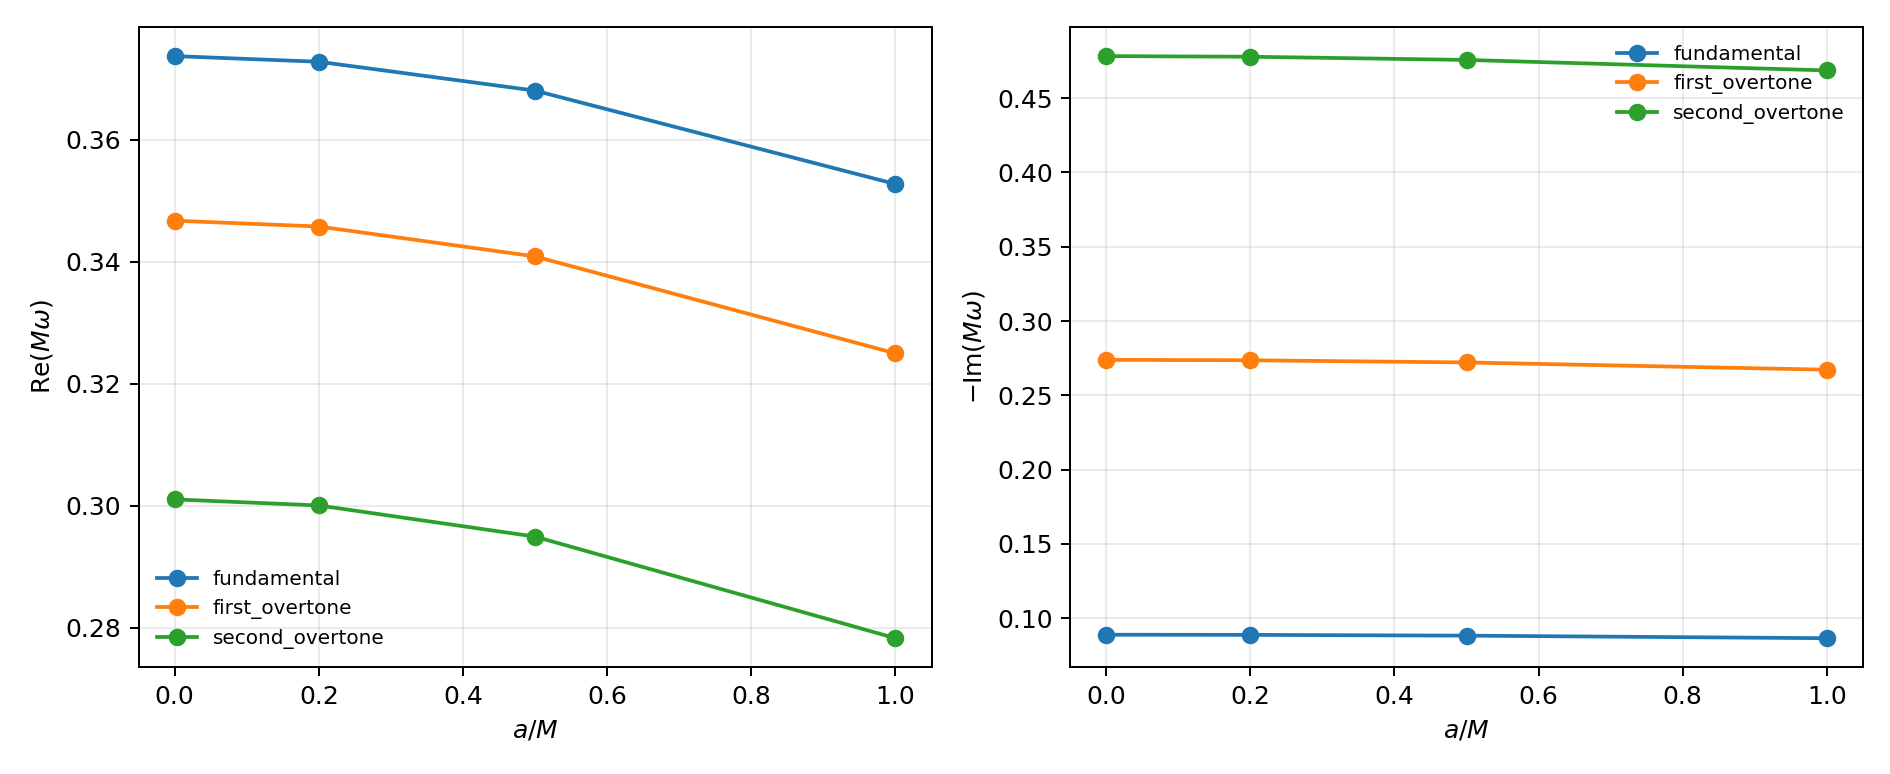
\includegraphics[width=\linewidth]{figures/figure2_mode_trajectories_gravitational_l2.png}
\caption{Representative \(\ell=2\) conditional odd-parity mode trajectories
of the gauge-invariant inverse-Cowling effective-source model versus \(a/M\).
They are not predictions of an unspecified quantum nonspherical completion.}
\label{fig:gravitationaltrajectory}
\end{figure}

Figure~\ref{fig:axialpotentialcomparison} compares the inverse-Cowling
potential with the lapse-substitution potential in
Eq.~\eqref{eq:lapsecomparison}. At \(a/M=1\), the
maximum absolute correction is \(5.77\%\) of the new barrier height; over the
region where the new potential exceeds \(10^{-3}\) of its peak, the maximum
pointwise fractional correction is \(15.1\%\).  These definitions avoid a
spurious relative divergence at the horizon and infinity, where both
potentials vanish.

\begin{figure}[H]
\centering
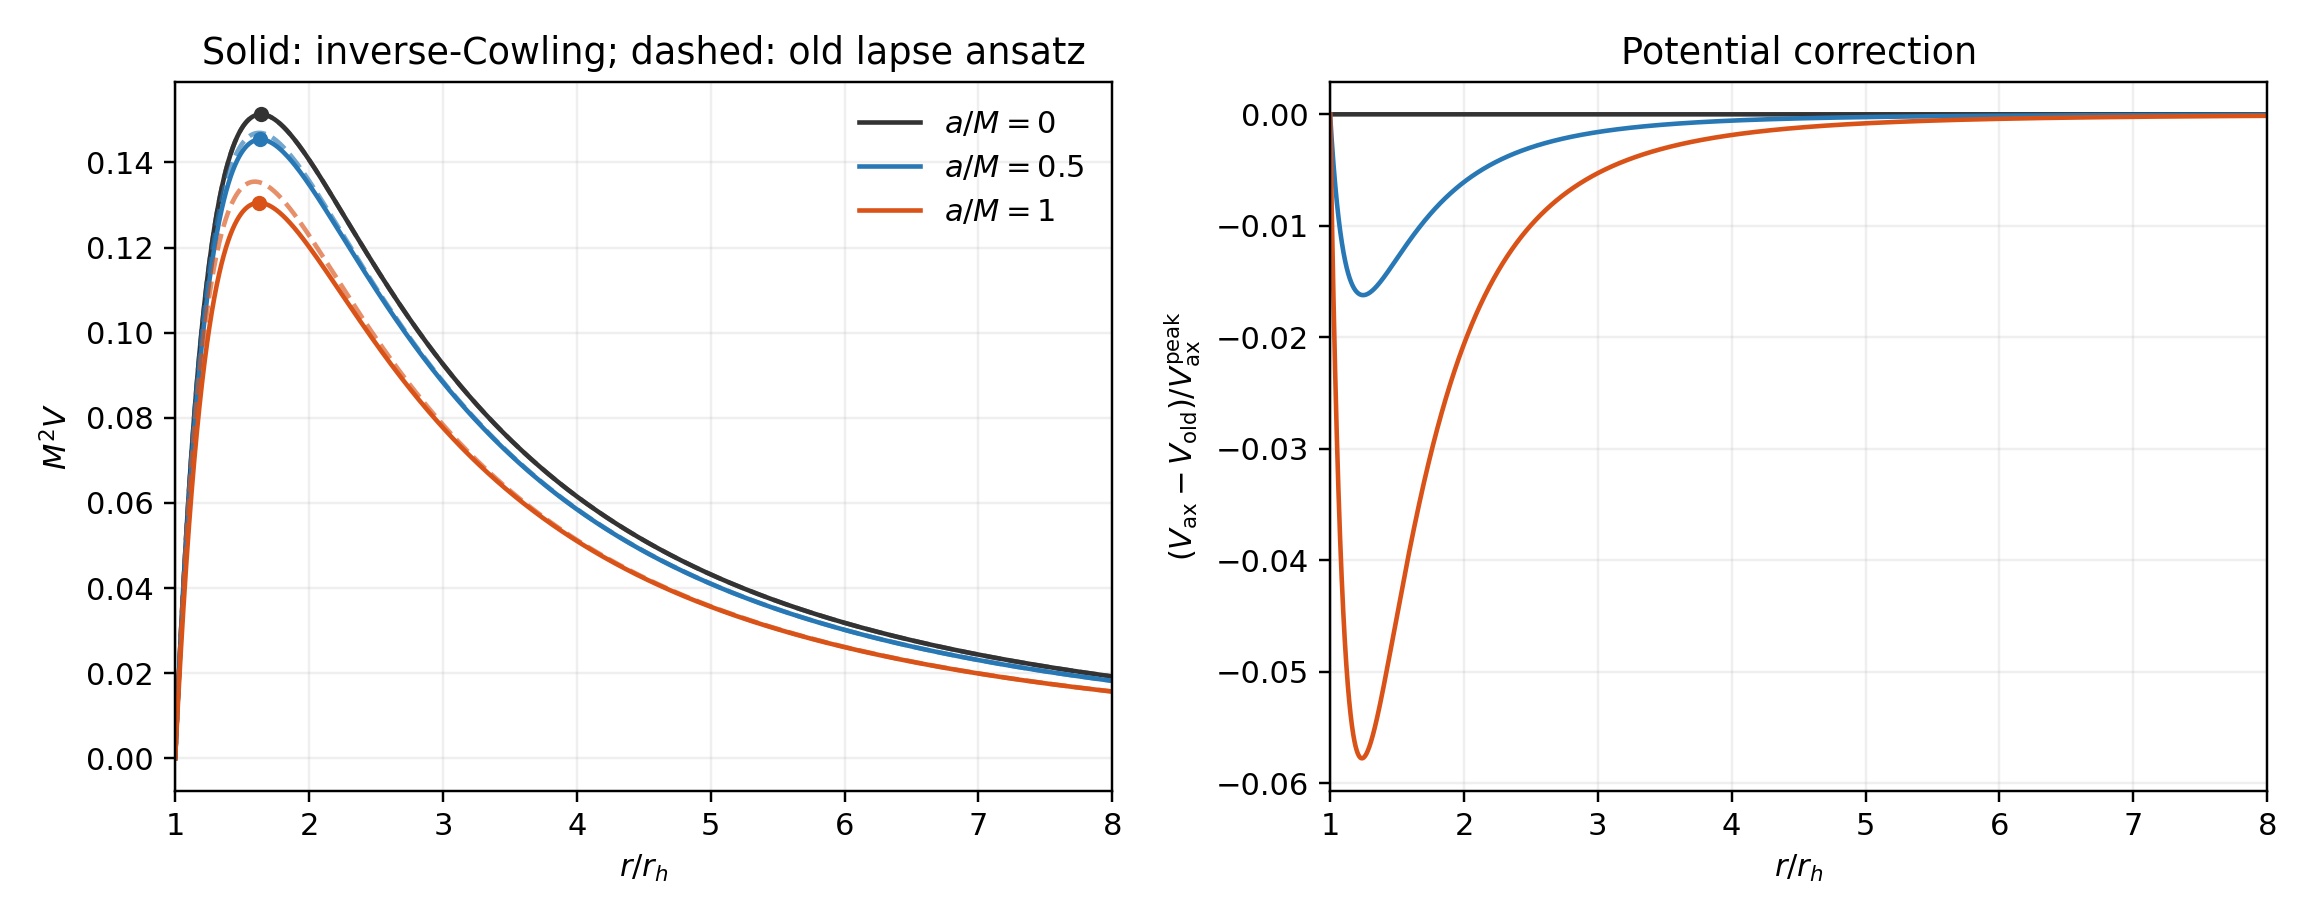
\includegraphics[width=\linewidth]{figures/figure2a_axial_potential_comparison.png}
\caption{Left: inverse-Cowling axial potential (solid) and the explicitly
defined lapse-substitution comparison potential (dashed) for \(\ell=2\);
circles mark the inverse-Cowling potential peaks and the vertical line marks
\(r=r_h\). Right: their
difference normalized by the new barrier height.}
\label{fig:axialpotentialcomparison}
\end{figure}

The same potential and mass normalization are used by the public 2026
high-precision Chebyshev calculation of Batic, Dutykh, and Sukaiti
\cite{BaticDutykhSukaiti2026}.  We compared all 18 overlapping
\(a/M=0.5,1\), \(\ell=2,3,4\), \(n=0,1,2\) entries.  The largest relative
difference is \(1.98\times10^{-13}\) for fundamentals,
\(3.80\times10^{-10}\) for first overtones, and \(1.62\times10^{-5}\) for
second overtones.  The last occurs at \(a/M=1,\ell=2,n=2\) and reinforces the
exploratory status of that tier.  The comparison, parameter conversion check,
public repository commit, and local source commit are recorded by
\texttt{scripts/audit\_axial\_model.py}.

As a stability diagnostic, the potential was minimized numerically outside
the horizon for every sampled \(a/M\) and \(\ell=2,3,4\).  It remained
non-negative and approached zero only at the two boundaries. The finite-spectrum
search was applied before the ordinary damped-mode window: all finite roots
satisfying \(\operatorname{Im}\omega>10^{-8}\) and \(|\omega|<5\) were retained
at \(N=32,48,64\), and persistence required agreement within \(10^{-4}\) at
all three sizes. Any persistent candidate was to be locally residual-refined
within radius \(0.02\) at \(N=64\) and accepted only if its polynomial backward
error was below \(10^{-8}\). No raw positive-imaginary root occurred, so the
refinement stage was not invoked and no growing candidate survived. Positivity
supplies the usual sufficient mode-stability
argument for this source-free one-dimensional problem.  For a hypothetical
mode with \(\operatorname{Im}\omega>0\), the QNM boundary conditions make the
radial solution decay at both asymptotic ends; multiplying the source-free
master equation by \(\Psi_{\mathrm{ax}}^*\), integrating, and using the
standard positive-energy identity excludes a growing mode when
\(V_{\mathrm{ax}}\geq0\) \cite{Boonserm2013}.  This statement applies only to
the inverse-Cowling model and does not establish stability under other
effective-source closures; the finite root search is an additional numerical
check.

Across the low-lying catalogue, the largest spectral--continued-fraction
difference is \(1.202\times10^{-5}\), for the axial \(\ell=2,n=2\) branch at
\(a/M=0.5\). The axial fundamentals are much more stable numerically. We keep
the \(n=1\) and \(n=2\) axial values because they show how the branches move,
but all axial modes inherit the inverse-Cowling assumption and the \(n=2\)
entries carry the additional overtone uncertainty familiar from KS studies
\cite{Bolokhov2025}.

\subsection{Catalogue-level deformation trends}

To isolate the effect of the KS deformation, we compare each branch with its
own Schwarzschild value at fixed \(M\). Both the real frequency and the damping
magnitude decrease monotonically on the sampled grid for every scalar branch.
The inverse-Cowling axial branches follow the same trend, although their
physical interpretation remains conditional on the frozen-source assumption.

At the upper endpoint of the sampled interval, \(a/M=1\), the scalar
\(\ell=2\) fundamental shifts are \(-7.29\%\) in
\(\operatorname{Re}(M\omega)\), \(-2.59\%\) in the damping magnitude
\(-\operatorname{Im}(M\omega)\), and \(7.17\%\) in the complex-plane
displacement \(|\Delta\omega|/|\omega(a=0)|\).  These are distinct quantities
and are not referred to interchangeably below.  Among the scalar fundamentals,
the \(\ell=4\) branch has the largest complex-plane displacement,
\(7.23\%\), while its real-part shift is \(-7.27\%\).  The scalar \(\ell=2\)
second overtone has a larger real-part shift, \(-9.16\%\), but is an
exploratory branch diagnostic.  The \(\ell=2\) trends are plotted in
Figure~\ref{fig:cataloguephysics}.

Within the closure-dependent axial fundamentals, the largest complex-plane
displacement is \(7.37\%\) for \(\ell=2\), with shifts of \(-7.54\%\) in the
real part and \(-2.80\%\) in damping magnitude.  This value is reported
separately because it depends on the frozen-source assumption, whereas the
scalar comparison above does not.

\begin{figure}[H]
\centering
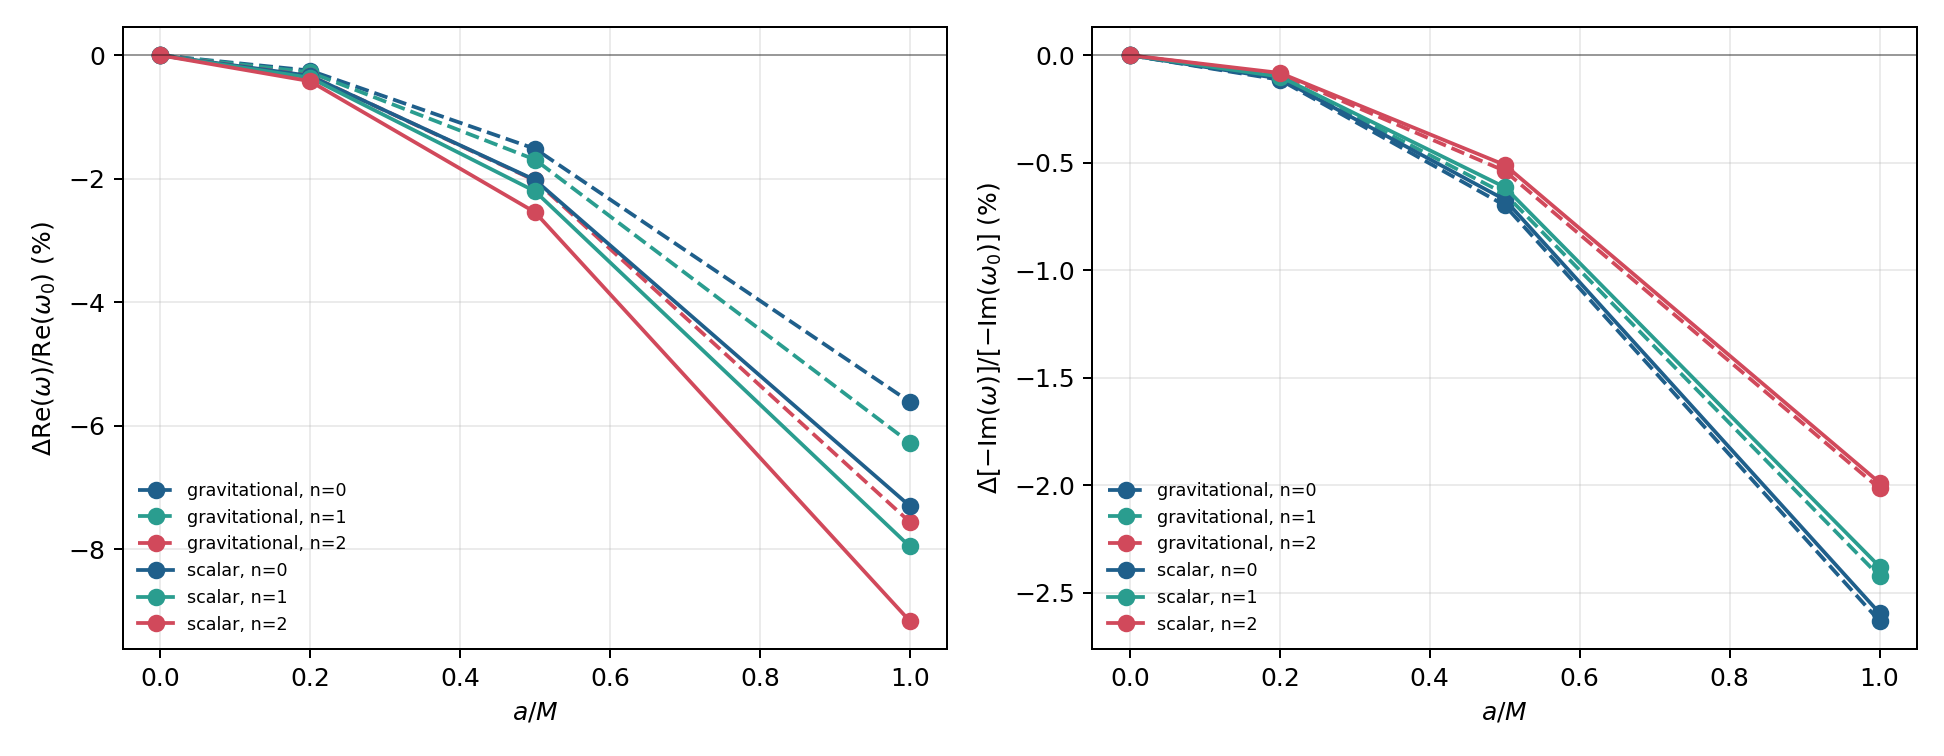
\includegraphics[width=\linewidth]{figures/figure3_catalogue_l2_fractional_shifts.png}
\caption{Schwarzschild-relative trends over the sampled interval for the
\(\ell=2\) branches. Solid curves show scalar modes and dashed curves show the
gauge-invariant inverse-Cowling axial modes.  The latter are conditional on the
closure stated in Section~2.1.}
\label{fig:cataloguephysics}
\end{figure}

The mild increase of the scalar fundamental displacement from \(\ell=2\) to
\(\ell=4\) is already visible in the effective-potential barrier.
Table~\ref{tab:potentialpeaks} reports the peak analysis
at \(a/M=1\).  The leading WKB proxy
\(\operatorname{Re}\omega\sim\sqrt{V_{\rm peak}}\) changes by \(-7.01\%\),
\(-7.13\%\), and \(-7.18\%\) for \(\ell=2,3,4\), respectively, mirroring the
modest multipole dependence of the computed fundamentals.  The curvature
change also grows slightly with \(\ell\), consistent with a weak
multipole-dependence in the damping. This is precisely the level of intuition
expected from leading WKB theory \cite{Ferrari1984,Konoplya2003}; the data do
not suggest a separate \(\ell=4\) mechanism.

\begin{table}[H]
\centering
\footnotesize
\begin{tabular}{rrrrr}
\toprule
\(\ell\) & \(r_{\rm peak}/M\) & \(\Delta V_{\rm peak}\) &
\(\Delta\sqrt{V_{\rm peak}}\) & \(\Delta|V''_{*,\rm peak}|\)\\
\midrule
2 & 3.25198574 & \(-13.5350\%\) & \(-7.0134\%\) & \(-17.7698\%\)\\
3 & 3.28015848 & \(-13.7535\%\) & \(-7.1310\%\) & \(-18.1334\%\)\\
4 & 3.29264164 & \(-13.8440\%\) & \(-7.1797\%\) & \(-18.2801\%\)\\
\bottomrule
\end{tabular}
\caption{Scalar effective-potential peak changes at \(a/M=1\), relative to
the Schwarzschild peak at the same \(\ell\).  Primes denote tortoise-coordinate
derivatives.  These diagnostics are generated by
\texttt{scripts/analyze\_scalar\_potential\_peaks.py} and provide only WKB
intuition; the QNM frequencies come from the Chebyshev and continued-fraction
calculations.}
\label{tab:potentialpeaks}
\end{table}

\subsection{Spectroscopy diagnostics}

At fixed mass, the shift has a straightforward spectroscopic meaning. The
decrease in \(\mathrm{Re}(M\omega)\) lowers the oscillation frequency, while the
decrease in \(-\mathrm{Im}(M\omega)\) lengthens the damping time. Following the
standard ringdown convention \cite{Berti2009,Berti2006}, we define
\begin{equation*}
Q=\frac{\operatorname{Re}\omega}{2[-\operatorname{Im}\omega]}.
\end{equation*}
If \(\tau=1/[-\operatorname{Im}\omega]\) is the time for the mode amplitude to
fall by a factor of \(e\), then the oscillation advances through \(2Q\) radians,
or \(Q/\pi\) cycles, during that time.  Thus \(Q\) measures how many oscillations
remain visible before damping substantially reduces the signal.
For the scalar \(\ell=2\) fundamental branch, the damping magnitude decreases by \(2.59\%\), corresponding to an approximate \(2.7\%\) increase in damping time. Because the oscillation frequency decreases by a larger fraction, \(Q\) decreases by \(4.83\%\): the scalar perturbation decays slightly more slowly, but it completes fewer oscillations per damping time.

Dimensionless mode ratios are useful because a common rescaling of the black-hole
mass cannot absorb them, which is why they play a central role in ringdown
spectroscopy \cite{Berti2006,Isi2019}. For the scalar \(\ell=2\) branch at
\(a/M=1\), the complex ratio \(\omega_0/\omega_1\) changes from
\(0.836060+0.324207\,\ii\) to \(0.823241+0.335659\,\ii\), a \(1.92\%\)
displacement in the complex-ratio plane. The corresponding
\(\omega_0/\omega_2\) ratio moves by \(3.56\%\). The branch-wise quantity
\(\mathrm{Re}(\omega)/[-\mathrm{Im}(\omega)]=2Q\) changes by \(-4.83\%\),
\(-5.71\%\), and \(-7.31\%\) for \(n=0,1,2\), respectively. The \(n=2\)
number is included only as an exploratory diagnostic. Figure~\ref{fig:spectroscopicratios}
collects these ratios and the fundamental \(Q(a/M)\) curve.

\begin{figure}[H]
\centering
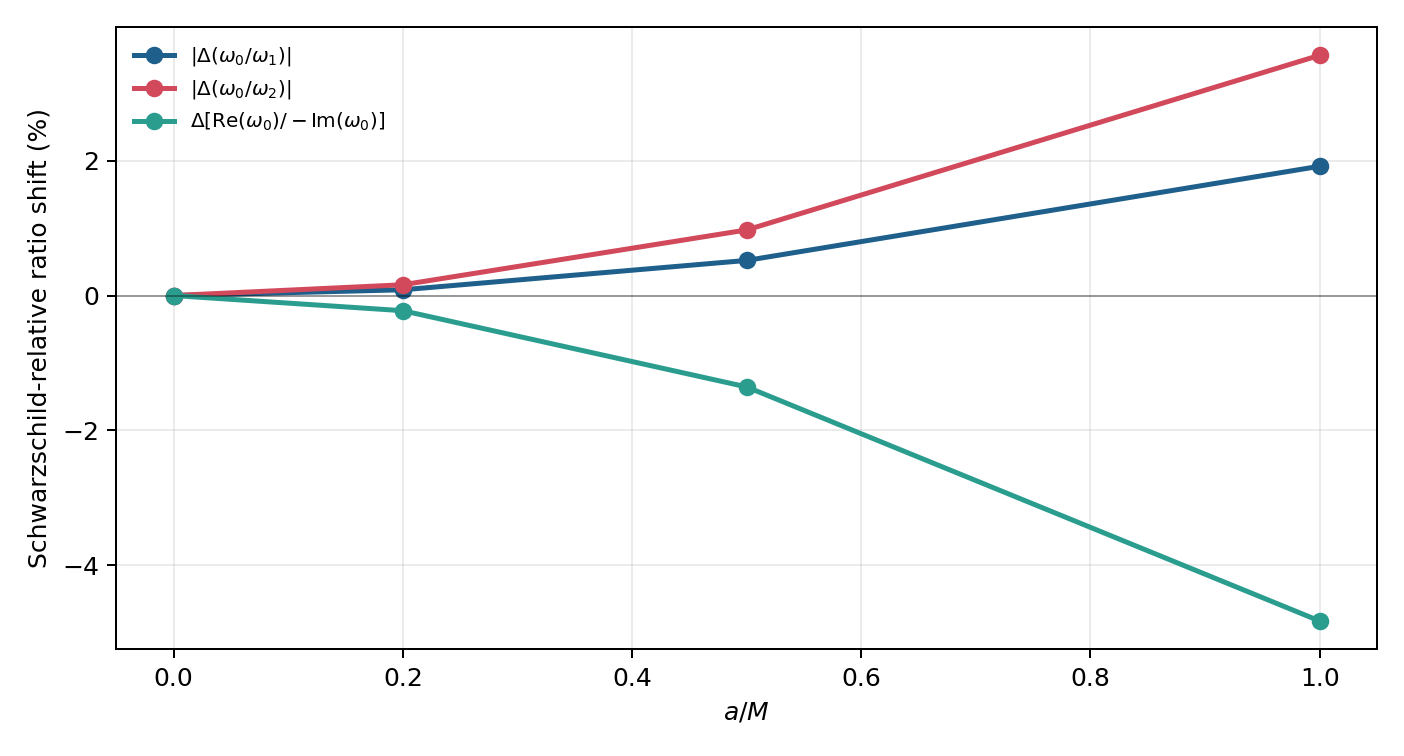
\includegraphics[width=\linewidth]{figures/figure4_catalogue_l2_spectroscopic_ratios.png}
\caption{Scalar \(\ell=2\) dimensionless spectroscopy diagnostics.  The left
panel shows Schwarzschild-relative changes in \(\omega_0/\omega_1\),
\(\omega_0/\omega_2\), and \(2Q\).  The right panel directly plots
\(Q=\operatorname{Re}\omega/[2(-\operatorname{Im}\omega)]\) for the robust
fundamental branch.  These quantities are catalogue diagnostics rather than an
observational forecast.}
\label{fig:spectroscopicratios}
\end{figure}
\FloatBarrier

The scalar \(\ell=2\) fundamental is consequently the best-controlled
spectroscopic quantity in this calculation. It is a quadrupolar test-field
mode, not the gravitational \(\ell=m=2\) ringdown mode measured by an
interferometer. Connecting the percent-level shifts found here to data would
require a gravitational waveform, detector-noise weighting, and a simultaneous
treatment of mass, spin, and mode amplitudes \cite{Berti2006,Isi2019}. Our
result is more modest but still physical: at fixed mass, the KS deformation
softens the low-lying scalar spectrum throughout the sampled interval.

\subsection{Comparison with existing KS literature}

Our results fit naturally into the existing KS literature. Konoplya studied
scalar, electromagnetic, and Dirac perturbations with WKB and time-domain
methods, together with scattering and shadow observables \cite{Konoplya2020}.
Bolokhov, Bronnikov, and Konoplya later used a Frobenius continued fraction to
show that KS overtones can respond much more strongly than the fundamental
mode \cite{Bolokhov2025}. The present calculation confirms the comparatively
smooth fundamental branches and quantifies them with a fixed-mass spectral
comparison.

Direct row-by-row numerical comparison requires care because the tabulated conventions and parameter normalizations differ. In particular, much of the earlier KS QNM literature fixes the horizon radius, while the catalogue here is organized at fixed mass scale and reports \(a/M\). For the lapse in Eq.~\eqref{eq:ksmetric}, a horizon-normalized parameter \(\beta=a/r_h\) corresponds to \(\alpha=a/M=2\beta/\sqrt{1-\beta^2}\), while \(r_h\omega=\sqrt{4+\alpha^2}\,M\omega\). Thus the \(a/M=1\) endpoint in this paper corresponds to \(a/r_h=1/\sqrt{5}\), not to a horizon-normalized \(a/r_h=1\) table row.

A direct numerical overlap is available for the scalar \(\ell=0,n=0\)
fundamental tabulated by Konoplya at fixed \(r_h=1\) \cite{Konoplya2020}.
After converting \(\beta=a/r_h\) to \(\alpha=a/M\), our horizon-scaled
frequencies agree with the published time-domain values at the
\(2.1\times10^{-3}\)--\(2.6\times10^{-3}\) level. Agreement with the
seventh-order WKB values is weaker, \(9.4\times10^{-3}\)--\(1.2\times10^{-2}\),
as expected for a low-\(\ell\) mode \cite{Konoplya2003,Konoplya2011}. This
comparison also makes clear why the normalization must be matched before two
KS tables are compared.

\begin{table}[H]
\centering
\footnotesize
\renewcommand{\arraystretch}{1.14}
\begin{tabular}{rrrrr}
\toprule
\(\beta=a/r_h\) & \(\alpha=a/M\) &
this work \(r_h\omega\) & Konoplya time-domain \(r_h\omega\) &
\(\Delta_{\mathrm{rel}}\)\\
\midrule
0.10 & 0.201008 & \(0.221242-0.210676\,\ii\) & \(0.221470-0.211440\,\ii\) & \(2.603\times10^{-3}\)\\
0.20 & 0.408248 & \(0.222244-0.213397\,\ii\) & \(0.222370-0.214200\,\ii\) & \(2.631\times10^{-3}\)\\
0.50 & 1.154701 & \(0.229462-0.235795\,\ii\) & \(0.230120-0.236200\,\ii\) & \(2.343\times10^{-3}\)\\
\bottomrule
\end{tabular}
\caption{Normalization-matched comparison with the scalar \(\ell=0,n=0\)
fixed-horizon table of Konoplya \cite{Konoplya2020}. The main catalogue starts
at \(\ell=2\); these rows test the parameter conversion and reproduce the
published scalar fundamental once the \(r_h\omega\) convention is matched.}
\label{tab:konoplyacomparison}
\end{table}

The overtone comparison with Bolokhov--Bronnikov--Konoplya is qualitative
because their published figures concern scalar \(\ell=0\) branches with
\(n=5,7,9\), whereas our catalogue covers \(\ell=2,3,4\) only through \(n=2\)
\cite{Bolokhov2025}. Both calculations nevertheless show the same hierarchy:
fundamentals vary smoothly, while overtones are more deformation-sensitive and
more demanding numerically. Our additional results are the fixed-mass branch
comparison, the quality-factor and mode-ratio shifts, and the singular-value
diagnostics.
\FloatBarrier

\subsection{Reported scalar rows}

Table~\ref{tab:spectralresults} collects the scalar rows used in the numerical
comparison and separates the time-domain orientation from the frequency-domain
values discussed in the text.

\begin{table}[H]
\centering
\footnotesize
\renewcommand{\arraystretch}{1.16}
\begin{tabular}{lrllrrrr}
\toprule
\(a/M\) & \(N\) & mode & status &
\(\mathrm{Re}(M\omega_{\mathrm{fit}})\) &
\(\mathrm{Re}(M\omega_{\mathrm{pencil}})\) &
\(\mathrm{Re}(M\omega_{\mathrm{spec}})\) &
\(\mathrm{Im}(M\omega_{\mathrm{spec}})\)\\
\midrule
0.0 & 96 & fundamental & high-\(N\) & 0.48364248 & 0.48365353 & 0.48364387 & -0.09675878\\
0.0 & 32 & first overtone & cross-validated & -- & -- & 0.46385058 & -0.29560394\\
0.2 & 96 & fundamental & high-\(N\) & 0.48203239 & 0.48204305 & 0.48203369 & -0.09665386\\
0.2 & 32 & first overtone & cross-validated & -- & -- & 0.46216559 & -0.29531130\\
0.5 & 96 & fundamental & high-\(N\) & 0.47388656 & 0.47389459 & 0.47388693 & -0.09610918\\
0.5 & 32 & first overtone & cross-validated & -- & -- & 0.45364275 & -0.29379018\\
1.0 & 96 & fundamental & high-\(N\) & 0.44836165 & 0.44836213 & 0.44836241 & -0.09424818\\
1.0 & 32 & first overtone & cross-validated & -- & -- & 0.42697149 & -0.28857291\\
\bottomrule
\end{tabular}
\caption{Scalar frequency comparison. Fundamental branches are reported at
\(N=96\); the cross-validated low-lying first overtones at \(N=32\) are quoted
on that grid. Displayed decimals identify the branches; the supported precision
is determined from spectral convergence and the continued fraction, not from
the residual alone. High-\(N\) overtone tracking is retained only as an
exploratory diagnostic.}
\label{tab:spectralresults}
\end{table}

\subsection{Residual diagnostics}

Table~\ref{tab:residualdiagnostics} reports scale-aware residual diagnostics
associated with the same scalar rows.  The raw smallest singular value answers
``how close is this matrix to having a null vector?'' but changes if the entire
equation is multiplied by a constant.  The polynomial backward error removes
that arbitrary overall scale.  It estimates the smallest relative perturbation
of the coefficient matrices that would make the reported frequency an exact
eigenvalue of the finite polynomial problem.  It is
\begin{equation}
\eta_{\mathrm{back}}(\omega)=
\frac{\sigma_{\min}[P_N(\omega)]}
{\lVert A_0\rVert_2+|\omega|\lVert A_1\rVert_2+|\omega|^2\lVert A_2\rVert_2}.
\label{eq:backwarderror}
\end{equation}

\begin{table}[H]
\centering
\footnotesize
\renewcommand{\arraystretch}{1.14}
\begin{tabular}{lrlrrr}
\toprule
\(a/M\) & \(N\) & mode & dim & \(\sigma_{\min}(P_N)\) & \(\eta_{\mathrm{back}}\)\\
\midrule
0.0 & 96 & fundamental & 96 & \(1.036\times10^{-19}\) & \(4.542\times10^{-22}\)\\
0.0 & 32 & first overtone & 32 & \(4.271\times10^{-19}\) & \(1.713\times10^{-20}\)\\
0.2 & 96 & fundamental & 96 & \(8.244\times10^{-21}\) & \(3.625\times10^{-23}\)\\
0.2 & 32 & first overtone & 32 & \(3.123\times10^{-19}\) & \(1.256\times10^{-20}\)\\
0.5 & 96 & fundamental & 96 & \(5.098\times10^{-20}\) & \(2.272\times10^{-22}\)\\
0.5 & 32 & first overtone & 32 & \(3.598\times10^{-19}\) & \(1.468\times10^{-20}\)\\
1.0 & 96 & fundamental & 96 & \(4.017\times10^{-20}\) & \(1.873\times10^{-22}\)\\
1.0 & 32 & first overtone & 32 & \(1.096\times10^{-19}\) & \(4.696\times10^{-21}\)\\
\bottomrule
\end{tabular}
\caption{Residual diagnostics for the reported spectral branches.  Both
quantities are evaluated by SVD on the raw, unscaled polynomial matrices; the
row/column equilibration used to generate eigenvalue candidates is not used
here.  Backward error is scale aware but is still interpreted together with
spectral-size and continued-fraction convergence.}
\label{tab:residualdiagnostics}
\end{table}

Hermiticity means \(R_N=R_N^\dagger\), and positive semidefiniteness means
\(v^\dagger R_Nv\geq0\) for every vector \(v\).  Both follow algebraically from
\(R_N=P_N^\dagger P_N\), up to floating-point roundoff; they are not presented
as empirical validation.  The automated tests instead check their numerical
implementation, Schwarzschild recovery, scaling invariance of the selected
root, the inverse-Cowling axial potential, and the numerically distinct validation paths.

\subsection{Local singular-value pseudospectral diagnostics of the scalar fundamental mode}

An eigenvalue table tells us where a mode is located but not how sharply that
location is defined.  This distinction matters for QNMs because outgoing
boundary conditions make the radial operator non-self-adjoint: its
eigenfunctions need not be orthogonal, and small operator perturbations can
move eigenvalues by much more than they would in a self-adjoint problem.  A
pseudospectrum addresses this by evaluating the residual throughout a region
of the complex-frequency plane rather than only at the eigenvalue.

The same residual operator therefore gives a local finite-dimensional
normalized singular-value pseudospectral diagnostic around a branch that has
already been cross-validated by the collocation-independent continued-fraction
calculation.  Following the
singular-value viewpoint used in black-hole pseudospectrum studies
\cite{Jaramillo2021,Cao2024}, we define
\begin{equation}
\eta_N(\omega)=\frac{\sigma_{\min}(P_N(\omega))}{\sigma_{\max}(P_N(\omega))}.
\end{equation}
The denominator removes a common matrix scale, so \(\eta_N\) compares the
weakest and strongest stretching directions of the matrix.  Small
\(\eta_N\) means that at least one normalized wavefunction nearly satisfies
the discretized equation.  Contours of equal \(\eta_N\) are therefore level
sets of ``almost-solutions.''  A narrow set indicates a sharply localized
root; a broad set indicates that a wider range of nearby frequencies produces
small relative residuals.  This is what the diagnostic gives us: a map of
local spectral sensitivity, complementary to the single best-fit frequency.
It is used here only for the finite Chebyshev matrices on the scalar
\(\ell=2,n=0\) branch.

Figure~\ref{fig:pseudocontours} shows contours of \(\log_{10}\eta_N\) around the residual-minimized scalar fundamental frequencies for \(a/M=0,0.2,0.5,1.0\), using \(N=64\), an \(81\times81\) grid, and a square half-width \(0.025\) in the complex \(M\omega\) plane. The contour centers agree with the Leaver frequencies to at worst \(6.816\times10^{-12}\) in relative difference, so the plotted basins are attached to the validated scalar branch.

The logarithm is used because the residual spans many orders of magnitude:
for example, \(\log_{10}\eta_N=-10\) means that the weakest matrix action is
one part in \(10^{10}\) of the strongest.  The white cross in each panel marks
the local residual minimum.  The surrounding contour shape, not the cross,
contains the new information supplied by the pseudospectrum.

\begin{figure}[H]
\centering
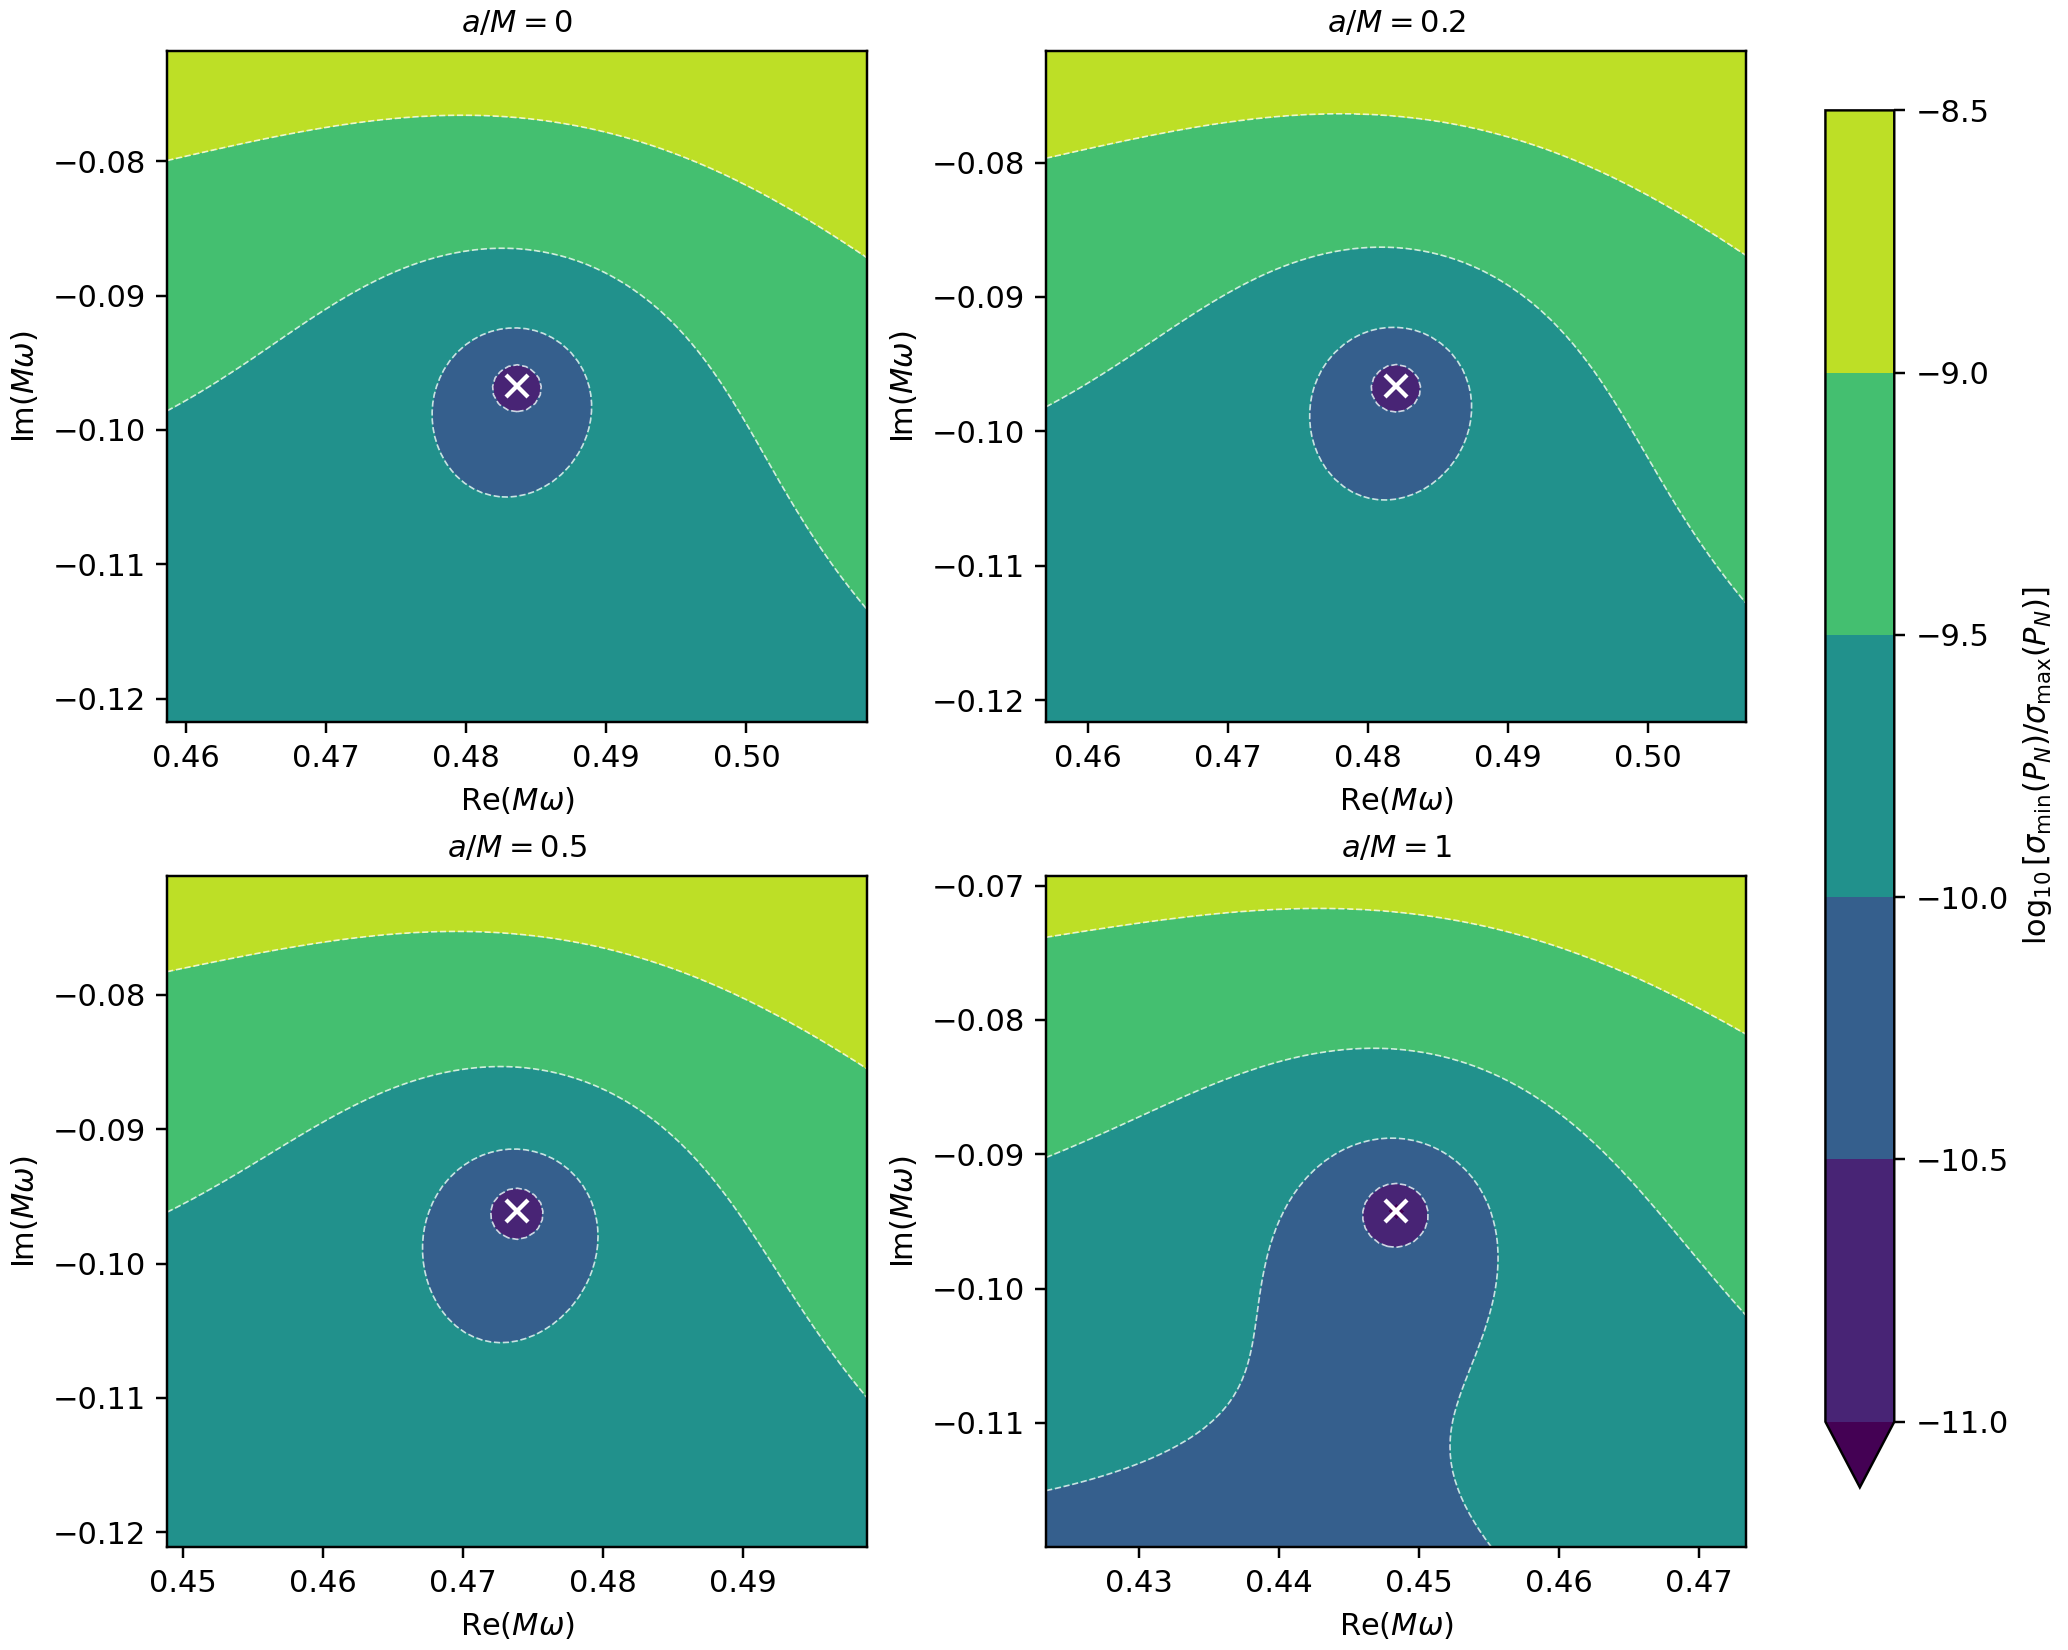
\includegraphics[width=\linewidth]{figures/figure5_scalar_l2_pseudospectrum_contours.png}
\caption{Finite-dimensional scalar \(\ell=2,n=0\) singular-value pseudospectral contours for the relative residual \(\eta_N=\sigma_{\min}(P_N)/\sigma_{\max}(P_N)\) at \(N=64\). White crosses mark the residual-minimized QNM locations. The panels show that the local small-\(\eta_N\) basin broadens as \(a/M\) increases.}
\label{fig:pseudocontours}
\end{figure}

Quantile and area diagnostics turn the contour picture into numbers.  A
\(p\)-quantile is the value below which a fraction \(p\) of all sampled grid
values lies.  Thus \(q_{10}\) characterizes the deepest \(10\%\) of the
residual landscape, while \(q_{50}\) is its median.  The area fraction below a
fixed threshold measures how much of the chosen window behaves as an
almost-solution.  Lower-case \(q_p\) distinguishes this statistic from the QNM
quality factor \(Q\).  At \(N=64\), \(-q_{10}\) rises from \(9.898\) at
\(a/M=0\) to \(10.060\) at \(a/M=1\), while \(-q_{50}\) rises from \(9.574\)
to \(9.710\).  The area fraction satisfying
\(\log_{10}\eta_N\le -10\) grows from \(4.36\%\) to \(22.07\%\), a factor
of \(5.06\).  In plain terms, the low-residual neighborhood occupies more of
the same local frequency window after deformation.  The upper-interval
contour is window-limited, so the area is used only as a local diagnostic.
These diagnostics are plotted in Figure~\ref{fig:pseudosensitivity}.

\begin{figure}[H]
\centering
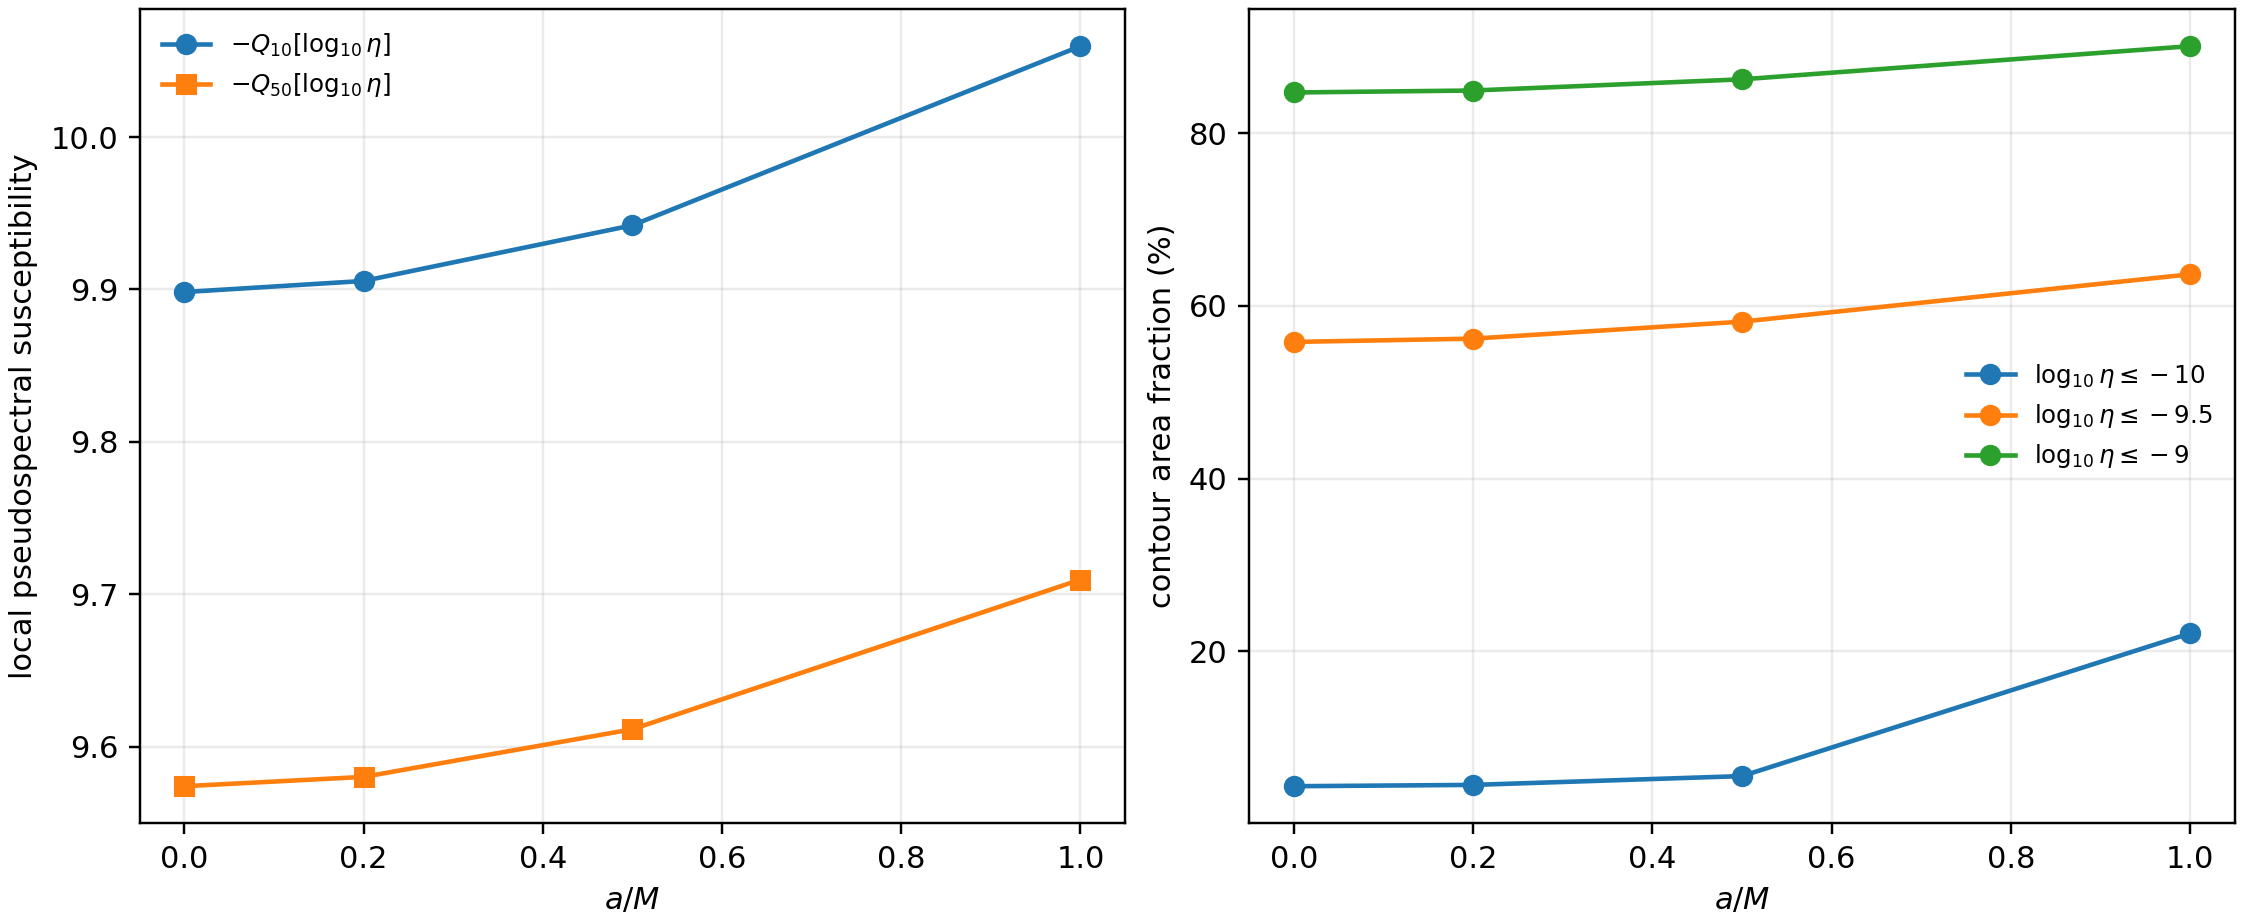
\includegraphics[width=\linewidth]{figures/figure6_scalar_l2_pseudospectrum_sensitivity.png}
\caption{Scalar \(\ell=2,n=0\) singular-value pseudospectral diagnostics at \(N=64\). Left: the normalized singular-value quantiles change with \(a/M\). Right: fixed-threshold contour area fractions also grow; the deepest endpoint contour is window-limited and is used only as a local diagnostic.}
\label{fig:pseudosensitivity}
\end{figure}

The sign of the quantile trend is stable under the tested spectral sizes. As shown in Figure~\ref{fig:pseudoresolution}, the \(a/M=0\) to \(a/M=1\) gain in \(-q_{10}\) is \(0.097\), \(0.130\), and \(0.161\) for \(N=32,48,64\), respectively. Thus, within the present residual normalization, scalar fundamental softening is associated with increasing local pseudospectral sensitivity.  This does not mean that the mode becomes unstable: instability would require a mode with \(\operatorname{Im}\omega>0\).  Nor is the contour width an observational error bar.  It measures sensitivity of the chosen finite operator and norm.

\begin{figure}[H]
\centering
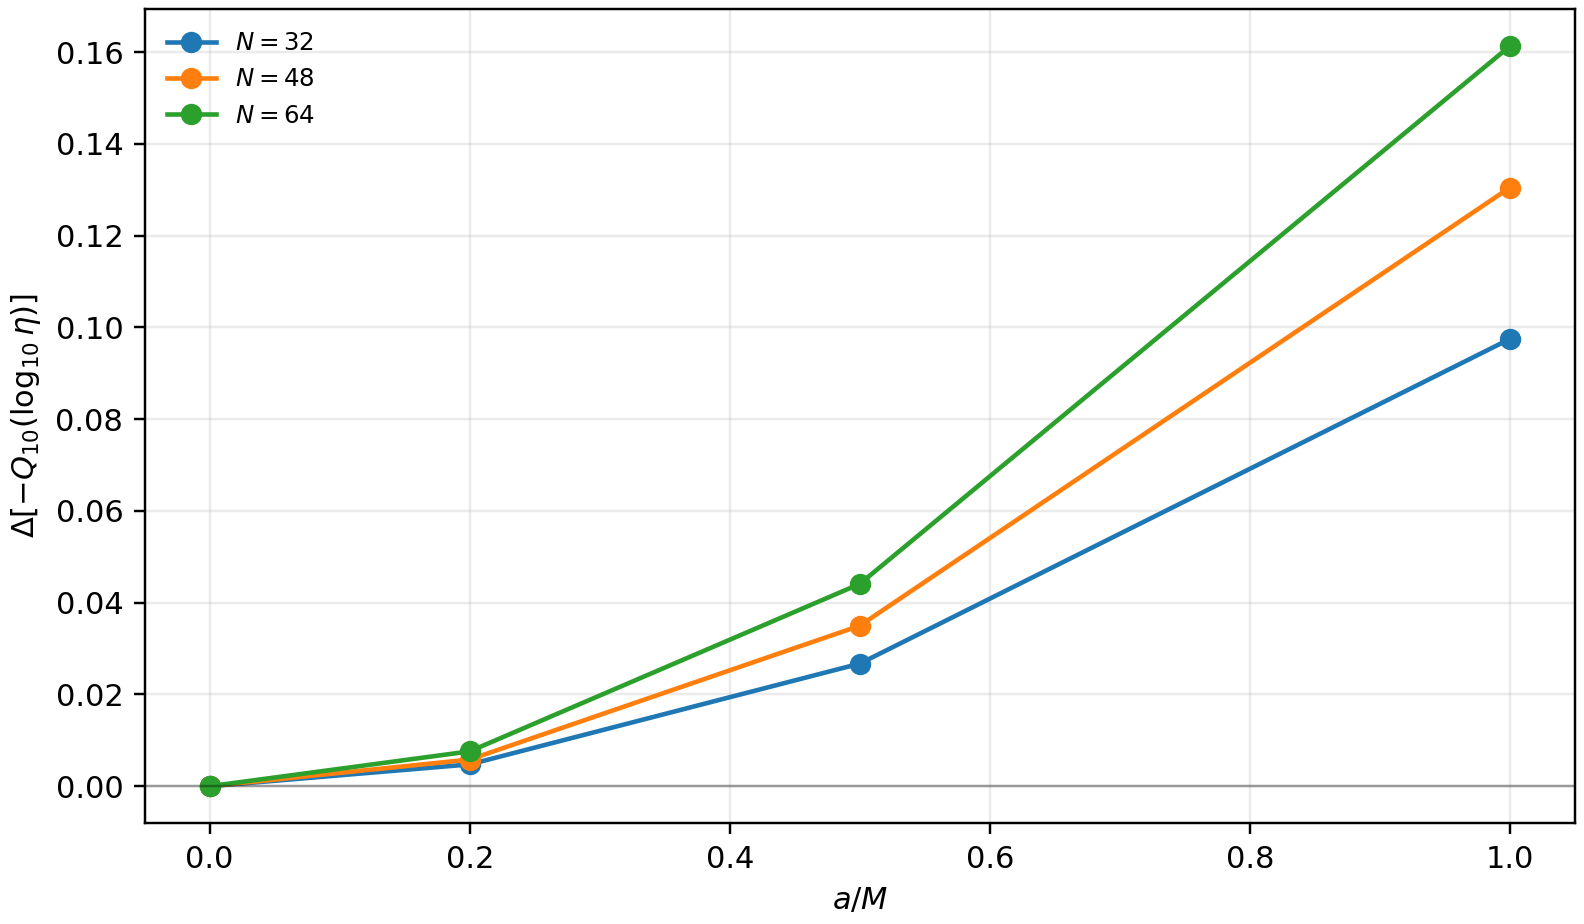
\includegraphics[width=0.82\linewidth]{figures/figure7_scalar_l2_pseudospectrum_resolution_check.png}
\caption{Finite-\(N\) check for the scalar \(\ell=2,n=0\) singular-value pseudospectral trend. The plotted quantity is the increase in \(-q_{10}(\log_{10}\eta_N)\) relative to the Schwarzschild value at the same \(N\). The successive increase across the sampled \(a/M\) grid is stable for \(N=32,48,64\), although the absolute contour levels remain resolution dependent.}
\label{fig:pseudoresolution}
\end{figure}

The dependence on grid density, frequency window, and spectral size is summarized in
Table~\ref{tab:pseudorobustness}.  It varies one numerical control at a time
around the \(N=64\), \(121^2\)-grid, half-width-\(0.025\) reference.  The
endpoint change remains positive in all seven configurations and spans
\(0.1002\)--\(0.1647\).  The sign and order of magnitude are therefore robust,
whereas the third decimal of a single-window result has no physical
significance.

\begin{table}[H]
\centering
\footnotesize
\begin{tabular}{lrrrr}
\toprule
test & \(N\) & grid & half-width &
\(\Delta[-q_{10}(\log_{10}\eta_N)]\)\\
\midrule
grid & 64 & \(81^2\) & 0.025 & 0.1613\\
grid & 64 & \(121^2\) & 0.025 & 0.1603\\
grid & 64 & \(161^2\) & 0.025 & 0.1607\\
window & 64 & \(121^2\) & 0.020 & 0.1396\\
window & 64 & \(121^2\) & 0.030 & 0.1647\\
spectral size & 32 & \(121^2\) & 0.025 & 0.1002\\
spectral size & 48 & \(121^2\) & 0.025 & 0.1287\\
\bottomrule
\end{tabular}
\caption{Robustness of the scalar-fundamental endpoint change in
\(-q_{10}(\log_{10}\eta_N)\) between \(a/M=0\) and \(a/M=1\). Every configuration gives the same positive
sign and comparable magnitude.  Full-precision values are generated by
\texttt{scripts/audit\_pseudospectrum\_robustness.py}.}
\label{tab:pseudorobustness}
\end{table}

\FloatBarrier
\section{Discussion}

The scalar calculation gives a direct relation between the deformed geometry
and the ringing it supports.  Increasing \(a/M\) at fixed mass moves both the
horizon and the peak of the scalar barrier outward.  At the same time the
barrier becomes lower and less sharply curved in the tortoise coordinate.  A
wave localized near that peak therefore oscillates at a lower frequency and
leaks away more slowly.  This is the physical origin of the systematic
softening of the scalar spectrum, rather than a numerical rescaling of an
otherwise unchanged Schwarzschild mode.

For the scalar \(\ell=2\) fundamental at \(a/M=1\), the pitch decreases by
\(7.29\%\) and the damping magnitude by \(2.59\%\).  Equivalently, the damping
time grows by approximately \(2.7\%\).  Since the oscillation slows more than
the envelope decay, the quality factor falls by \(4.83\%\): the perturbation
lives slightly longer in time but executes fewer cycles before fading.  The
weak \(\ell\)-dependence follows the height and curvature of the scalar barrier
as expected from WKB theory \cite{Ferrari1984,Konoplya2003}.  These results put
the qualitative softening found in earlier KS calculations on a fixed-mass,
low-lying spectral footing \cite{Konoplya2020,Bolokhov2025}.

The agreement between Chebyshev and Frobenius calculations is strongest for the
fundamentals and remains excellent for the first overtones at \(N=32\). The
second overtones are less regular, with a maximum discrepancy of
\(1.202\times10^{-5}\) on the axial \(\ell=2\) branch. This behavior is not
surprising: highly damped modes are well known to require greater care in both
continued-fraction and spectral calculations \cite{Leaver1985,Nollert1993,Bolokhov2025,Chen2025}.
For this reason the scalar fundamentals are the quantitative core of the paper,
the scalar \(n=1\) modes are cross-validated low-lying first overtones at
\(N=32\), and the \(n=2\) values are best regarded as indications of branch
motion.

The axial calculation asks a different question.  It describes how an
odd-parity metric disturbance rings when the spherical quantum-corrected
background is retained but its effective quantum source is not allowed to
develop an independent odd-parity motion.  The resulting master variable is
gauge invariant, so its motion is not a coordinate artifact, but the
frozen-source assumption is still physical input.  The axial frequencies are
therefore useful conditional predictions of that model, not universal KS
gravitational-wave frequencies.

Finally, the local singular-value contours broaden with \(a/M\) on the scalar
\(\ell=2,n=0\) branch.  In physical terms, nearby complex frequencies become
less sharply distinguishable in the finite spectral representation as the
geometry is deformed.  Similar pseudospectral broadening has been used to
expose the sensitivity of non-self-adjoint black-hole spectra
\cite{Jaramillo2021,Cao2024}.  Because our calculation is finite dimensional
and local in the complex-frequency plane, this is a sensitivity diagnostic,
not evidence for a continuum instability.

\subsection{Limitations and reproducibility}

\subsubsection{Interpretive boundaries}

The scalar calculation requires only the KS metric and the minimally coupled
Klein--Gordon equation, and is therefore the least model-dependent part of the
analysis \cite{Kazakov1994,Konoplya2020}. The axial master variable is gauge
invariant, but its homogeneous equation is obtained only after setting the
invariant odd effective-source amplitudes to zero
\cite{Gerlach1979,Gundlach1999,Karlovini2002}. The axial frequencies thus belong
to this inverse-Cowling model. Gauge invariance does not make the closure unique.

Nor should the percent-level shifts be read directly as detector forecasts.
Part of a dimensional frequency change is degenerate with the remnant mass,
and a measurement requires mode amplitudes, a waveform model, detector noise,
and covariances with mass and spin \cite{Berti2006,Berti2009,Isi2019}. The
dimensionless ratios reported above reduce the mass degeneracy but do not
replace such an analysis.

The pseudospectral plots are built from finite Chebyshev matrices rather than a
controlled infinite-dimensional KS operator. Normalizing by
\(\sigma_{\max}\) removes an overall matrix scale, but not the dependence on
discretization and norm. The robust statement is consequently limited to the
observed branch: for \(N=32,48,64\), the endpoint quantile change has the same
sign and comparable size. A continuum
pseudospectrum would require a separate operator-theoretic treatment
\cite{Jaramillo2021,Cao2024}.

Finally, the loss of monotonic Chebyshev convergence for the overtones prevents
us from extending the same precision statement to arbitrary \(n\). The
reported \(n=1\) frequencies are cross-validated low-lying first overtones at
\(N=32\); the \(n=2\) rows are included to show the emerging deformation trend,
and higher overtones are not considered. Table~\ref{tab:claimhierarchy}
summarizes these distinctions.

\begin{table}[!htbp]
\centering
\footnotesize
\renewcommand{\arraystretch}{1.16}
\setlength{\tabcolsep}{3pt}
\begin{tabularx}{\columnwidth}{>{\raggedright\arraybackslash}p{0.22\columnwidth}>{\raggedright\arraybackslash}p{0.25\columnwidth}>{\raggedright\arraybackslash}X}
\toprule
Branch & Numerical status & Physical interpretation \\
\midrule
Scalar \(n=0\) & Robust fundamental modes & Quantitative softening and spectroscopy results. \\
Scalar \(n=1\) & Cross-validated low-lying first overtones at \(N=32\) & Secondary diagnostics; high-\(N\) tracking remains exploratory. \\
Overtones \(n=2\) & Exploratory branch diagnostics & Qualitative deformation trends. \\
Axial rows & Conditional inverse-Cowling odd-parity modes & Gauge-invariant metric variable with frozen axial effective-source current. \\
\bottomrule
\end{tabularx}
\caption{Numerical and physical status of the reported branches. Scalar
fundamentals and first overtones are distinguished from exploratory second
overtones and closure-dependent axial modes.}
\label{tab:claimhierarchy}
\end{table}

\subsubsection{Reproducibility}

The implementation is reproducible from the accompanying repository:
\begin{center}
\url{https://github.com/adoolelomani2026/ks-qnm-spectral-residual-workflow}
\end{center}
The repository contains the Chebyshev spectral solver, the Leaver-style validation layer, catalogue-generation scripts, pseudospectrum diagnostics, generated tables, manuscript-supporting figures, and automated tests. The submission-facing commands are copied literally below.
\begin{verbatim}
pytest
python tests/test_qnm_algorithm.py --full
python scripts/run_hybrid_qnm_algorithm.py
python scripts/analyze_leaver_convergence.py
python scripts/analyze_solver_convergence.py
python scripts/analyze_scalar_potential_peaks.py
python scripts/audit_axial_model.py
python scripts/check_n128_spot.py
python scripts/analyze_pseudospectrum.py
python scripts/audit_pseudospectrum_robustness.py
python scripts/compare_konoplya2020_scalar_l0.py
\end{verbatim}
The first two commands run the fast and complete scalar/axial validation
suites.  The remaining commands regenerate the main results, convergence
audits, potential diagnostics, pseudospectrum data, and literature comparisons.
These commands write the CSV tables, Markdown summaries, and figures under \path{outputs/results/} and \path{outputs/figures/}. The package versions used for the regenerated outputs are recorded in \path{outputs/results/run_metadata.json}.

\section{Conclusion}

The main physical result is that the KS deformation softens the low-lying
test-scalar ringing at fixed mass.  The deformation pushes the effective
barrier outward and lowers its height and curvature.  The trapped scalar wave
therefore rings at a lower frequency and decays slightly more slowly.  For
\(\ell=2\) at \(a/M=1\), the oscillation frequency, damping magnitude, and
quality factor change by \(-7.29\%\), \(-2.59\%\), and \(-4.83\%\),
respectively.  The scalar perturbation consequently survives for a little
longer but completes fewer cycles during that time.  The dimensionless
\(\omega_0/\omega_1\) ratio moves by \(1.92\%\), confirming that the result is
not merely a common change of mass units.  This complements earlier WKB,
time-domain, and Frobenius studies of the same geometry
\cite{Konoplya2020,Bolokhov2025}.

At \(N=32\), the scalar fundamentals agree with the continued-fraction values
to \(7.92\times10^{-13}\) or better on the sampled deformation grid. The
\(N=96\) values used for the principal scalar convergence study lie on the
high-resolution plateau and differ from the continued-fraction values by
\(1.23\times10^{-11}\)--\(2.02\times10^{-10}\). The first overtones exhibit a
finite-precision optimum near \(N=32\) and are therefore quoted as
cross-validated low-lying first overtones at \(N=32\). The second overtones
show larger truncation and branch sensitivity and remain exploratory. This is
also why we make no claim about the highly damped spectrum, for which dedicated
analytic-continuation methods are better suited \cite{Chen2025}.

For odd-parity gravitational perturbations, the gauge-invariant master variable
obeys a sourced equation on a general spherical background
\cite{Gerlach1979,Gundlach1999,Karlovini2002}. Setting the invariant axial
effective-source current to zero gives the inverse-Cowling potential used here,
which differs from a simple lapse-deformed Regge--Wheeler potential. Its
frequencies provide a useful numerical comparison and agree closely with the
separate high-precision Chebyshev calculation of Batic, Dutykh, and Sukaiti
\cite{BaticDutykhSukaiti2026}, but their
physical meaning remains conditional on the frozen-source closure. A complete
nonspherical quantum theory of the KS source would be needed to remove that
assumption.

The local finite-\(N\) pseudospectral basin of the scalar fundamental broadens
with deformation, indicating greater local numerical sensitivity around the
resonance without implying a continuum instability.  The computational audits
support, rather than replace, the physical conclusion: two numerically distinct
radial representations identify the same robust fundamental branches, while the
second overtones remain too fragile for equally strong claims
\cite{Leaver1985,Jansen2017,Jaramillo2021}.

\appendix
\section{Schwarzschild branch-identification seeds}
\label{sec:schwarzschildseeds}

Table~\ref{tab:schwarzschildseeds} records every initial target used at
\(a/M=0\). Each is a literature value: no seed was selected manually and no
continued-fraction result was used as an initial Schwarzschild seed. For each
\((s,\ell,n)\), the code chooses the nearest distinct \(N=32\) Chebyshev
candidate and refines it with the continued fraction. The accepted
continued-fraction root then becomes the target at the next value of \(a/M\).
The machine-readable table, including a provenance field for every row, is
generated as \path{outputs/results/schwarzschild_branch_seeds.csv}.

\begin{table}[H]
\centering
\scriptsize
\setlength{\tabcolsep}{4pt}
\begin{tabular}{lrrrr}
\toprule
sector & \(\ell\) & \(n\) & \(\operatorname{Re}(M\omega_{\rm seed})\) & \(\operatorname{Im}(M\omega_{\rm seed})\)\\
\midrule
scalar & 2 & 0 & 0.483643872211 & -0.096758775978\\
scalar & 2 & 1 & 0.463850579020 & -0.295603936988\\
scalar & 2 & 2 & 0.430544 & -0.508558\\
scalar & 3 & 0 & 0.675366 & -0.096500\\
scalar & 3 & 1 & 0.660671 & -0.292285\\
scalar & 3 & 2 & 0.633626 & -0.496008\\
scalar & 4 & 0 & 0.867416 & -0.096392\\
scalar & 4 & 1 & 0.855808 & -0.290876\\
scalar & 4 & 2 & 0.833692 & -0.490325\\
axial & 2 & 0 & 0.373671680 & -0.088962320\\
axial & 2 & 1 & 0.346710996 & -0.273914876\\
axial & 2 & 2 & 0.301053454 & -0.478276983\\
axial & 3 & 0 & 0.599443288 & -0.092703048\\
axial & 3 & 1 & 0.582643804 & -0.281298113\\
axial & 3 & 2 & 0.551684837 & -0.479092791\\
axial & 4 & 0 & 0.809178378 & -0.094163961\\
axial & 4 & 1 & 0.796631 & -0.284334\\
axial & 4 & 2 & 0.772695 & -0.479900\\
\bottomrule
\end{tabular}
\caption{Literature tracking targets used to identify the Schwarzschild
branches. The scalar \(\ell=2,n=0\) value is pinned to Table~I of Cavalcante
and da Cunha \cite{Cavalcante2021}; the remaining branch targets are drawn from
the Schwarzschild tabulations reviewed by Berti, Cardoso, and Starinets
\cite{Berti2009}. Rounded entries identify branches and are not treated as
high-precision accuracy standards.}
\label{tab:schwarzschildseeds}
\end{table}

\section*{Acknowledgements and declarations}

\noindent\textbf{Funding.}
No funding was received to assist with the preparation of this manuscript.

\noindent\textbf{Competing interests.}
The author declares no competing interests.

\noindent\textbf{Data availability.}
The numerical data generated in this study, including catalogue rows, spectroscopy diagnostics, and scalar pseudospectrum grids, are available from the accompanying code repository and supplementary output files at \url{https://github.com/adoolelomani2026/ks-qnm-spectral-residual-workflow}.

\noindent\textbf{Code availability.}
The code used to generate the spectral results, Leaver validation, catalogue tables, pseudospectrum diagnostics, and figures is available from the accompanying repository at \url{https://github.com/adoolelomani2026/ks-qnm-spectral-residual-workflow}.

\noindent\textbf{Author contribution.}
Adel H. Al-Yoorby conceived the study, developed the numerical implementation, generated and analyzed the data, prepared the figures and tables, and wrote the manuscript.

\noindent\textbf{Ethics approval.}
Not applicable.

\noindent\textbf{Consent to participate.}
Not applicable.

\noindent\textbf{Consent for publication.}
Not applicable.

\noindent\textbf{Use of AI tools.}
Artificial intelligence (AI) tools were used during preparation of this work.
The author executed the calculations, checked cited claims against the primary
sources, reviewed the derivations and numerical outputs, and takes
responsibility for the final content.

\begin{thebibliography}{99}

\bibitem{Regge1957}
T. Regge and J. A. Wheeler,
``Stability of a Schwarzschild singularity,''
\emph{Physical Review} \textbf{108}, 1063--1069 (1957).
\url{https://doi.org/10.1103/PhysRev.108.1063}

\bibitem{Gerlach1979}
U. H. Gerlach and U. K. Sengupta,
``Gauge-invariant perturbations on most general spherically symmetric
space-times,''
\emph{Physical Review D} \textbf{19}, 2268--2272 (1979).
\url{https://doi.org/10.1103/PhysRevD.19.2268}

\bibitem{Gundlach1999}
C. Gundlach and J. M. Mart\'inez-Garc\'ia,
``Gauge-invariant and coordinate-independent perturbations of stellar
collapse. I. The interior,''
\emph{Physical Review D} \textbf{61}, 084024 (2000).
\url{https://doi.org/10.1103/PhysRevD.61.084024}

\bibitem{Karlovini2002}
M. Karlovini,
``Axial perturbations of general spherically symmetric spacetimes,''
\emph{Classical and Quantum Gravity} \textbf{19}, 2125--2140 (2002).
\url{https://doi.org/10.1088/0264-9381/19/8/305}

\bibitem{Boonserm2013}
P. Boonserm, T. Ngampitipan, and M. Visser,
``Regge--Wheeler equation, linear stability, and greybody factors for dirty
black holes,''
\emph{Physical Review D} \textbf{88}, 041502(R) (2013).
\url{https://doi.org/10.1103/PhysRevD.88.041502}

\bibitem{BaticDutykhSukaiti2026}
D. Batic, D. Dutykh, and M. E. Sukaiti,
``Quasinormal modes of the Kazakov--Solodukhin quantum-corrected black hole:
a spectral analysis,'' public manuscript and reproducibility repository (2026),
commit \nolinkurl{f53435ebdb8d1124d13bee75fa54972ac1613a03}, accessed 20 July 2026.
\url{https://github.com/dutykh/KS-quantum}

\bibitem{Vishveshwara1970}
C. V. Vishveshwara,
``Scattering of gravitational radiation by a Schwarzschild black-hole,''
\emph{Nature} \textbf{227}, 936--938 (1970).
\url{https://doi.org/10.1038/227936a0}

\bibitem{Kokkotas1999}
K. D. Kokkotas and B. G. Schmidt,
``Quasi-normal modes of stars and black holes,''
\emph{Living Reviews in Relativity} \textbf{2}, 2 (1999).
\url{https://doi.org/10.12942/lrr-1999-2}

\bibitem{Berti2009}
E. Berti, V. Cardoso, and A. O. Starinets,
``Quasinormal modes of black holes and black branes,''
\emph{Classical and Quantum Gravity} \textbf{26}, 163001 (2009).
\url{https://doi.org/10.1088/0264-9381/26/16/163001}

\bibitem{Konoplya2011}
R. A. Konoplya and A. Zhidenko,
``Quasinormal modes of black holes: From astrophysics to string theory,''
\emph{Reviews of Modern Physics} \textbf{83}, 793--836 (2011).
\url{https://doi.org/10.1103/RevModPhys.83.793}

\bibitem{Abbott2016Observation}
B. P. Abbott et al. (LIGO Scientific Collaboration and Virgo Collaboration),
``Observation of gravitational waves from a binary black hole merger,''
\emph{Physical Review Letters} \textbf{116}, 061102 (2016).
\url{https://doi.org/10.1103/PhysRevLett.116.061102}

\bibitem{Berti2006}
E. Berti, V. Cardoso, and C. M. Will,
``Gravitational-wave spectroscopy of massive black holes with the space interferometer LISA,''
\emph{Physical Review D} \textbf{73}, 064030 (2006).
\url{https://doi.org/10.1103/PhysRevD.73.064030}

\bibitem{Isi2019}
M. Isi et al.,
``Testing the no-hair theorem with GW150914,''
\emph{Physical Review Letters} \textbf{123}, 111102 (2019).
\url{https://doi.org/10.1103/PhysRevLett.123.111102}

\bibitem{Kazakov1994}
D. I. Kazakov and S. N. Solodukhin,
``On quantum deformation of the Schwarzschild solution,''
\emph{Nuclear Physics B} \textbf{429}, 153--176 (1994).
\url{https://doi.org/10.1016/S0550-3213(94)80045-6}

\bibitem{Berry2021}
T. Berry, A. Simpson, and M. Visser,
``Regularity of a general class of ``quantum deformed'' black holes,''
\emph{Universe} \textbf{7}, 165 (2021).
\url{https://doi.org/10.3390/universe7060165}

\bibitem{Konoplya2020}
R. A. Konoplya,
``Quantum corrected black holes: Quasinormal modes, scattering, shadows,''
\emph{Physics Letters B} \textbf{804}, 135363 (2020).
\url{https://doi.org/10.1016/j.physletb.2020.135363}

\bibitem{Bolokhov2025}
S. V. Bolokhov, K. A. Bronnikov, and R. A. Konoplya,
``Overtones' outburst and Hawking evaporation of Kazakov--Solodukhin quantum corrected black hole,''
\emph{Fortschritte der Physik} \textbf{73}, 2400187 (2025).
\url{https://doi.org/10.1002/prop.202400187}

\bibitem{Leaver1985}
E. W. Leaver,
``An analytic representation for the quasi-normal modes of Kerr black holes,''
\emph{Proceedings of the Royal Society of London A: Mathematical and Physical Sciences} \textbf{402}, 285--298 (1985).
\url{https://doi.org/10.1098/rspa.1985.0119}

\bibitem{Nollert1993}
H.-P. Nollert,
``Quasinormal modes of Schwarzschild black holes: The determination of
quasinormal frequencies with very large imaginary parts,''
\emph{Physical Review D} \textbf{47}, 5253--5258 (1993).
\url{https://doi.org/10.1103/PhysRevD.47.5253}

\bibitem{Schutz1985}
B. F. Schutz and C. M. Will,
``Black hole normal modes: A semianalytic approach,''
\emph{The Astrophysical Journal Letters} \textbf{291}, L33--L36 (1985).
\url{https://doi.org/10.1086/184453}

\bibitem{Iyer1987}
S. Iyer and C. M. Will,
``Black-hole normal modes: A WKB approach. I. Foundations and application of
a higher-order WKB analysis of potential-barrier scattering,''
\emph{Physical Review D} \textbf{35}, 3621--3631 (1987).
\url{https://doi.org/10.1103/PhysRevD.35.3621}

\bibitem{Ferrari1984}
V. Ferrari and B. Mashhoon,
``New approach to the quasinormal modes of a black hole,''
\emph{Physical Review D} \textbf{30}, 295--304 (1984).
\url{https://doi.org/10.1103/PhysRevD.30.295}

\bibitem{Konoplya2003}
R. A. Konoplya,
``Quasinormal behavior of the D-dimensional Schwarzschild black hole and higher order WKB approach,''
\emph{Physical Review D} \textbf{68}, 024018 (2003).
\url{https://doi.org/10.1103/PhysRevD.68.024018}

\bibitem{Cho2010}
H. T. Cho, A. S. Cornell, J. Doukas, and W. Naylor,
``Black hole quasinormal modes using the asymptotic iteration method,''
\emph{Classical and Quantum Gravity} \textbf{27}, 155004 (2010).
\url{https://doi.org/10.1088/0264-9381/27/15/155004}

\bibitem{Gundlach1994}
C. Gundlach, R. H. Price, and J. Pullin,
``Late-time behavior of stellar collapse and explosions. I. Linearized
perturbations,''
\emph{Physical Review D} \textbf{49}, 883--889 (1994).
\url{https://doi.org/10.1103/PhysRevD.49.883}

\bibitem{Hua1990}
Y. Hua and T. K. Sarkar,
``Matrix pencil method for estimating parameters of exponentially
damped/undamped sinusoids in noise,''
\emph{IEEE Transactions on Acoustics, Speech, and Signal Processing}
\textbf{38}, 814--824 (1990).
\url{https://doi.org/10.1109/29.56027}

\bibitem{Jansen2017}
A. Jansen,
``Overdamped modes in Schwarzschild-de Sitter and a Mathematica package for the numerical computation of quasinormal modes,''
\emph{The European Physical Journal Plus} \textbf{132}, 546 (2017).
\url{https://doi.org/10.1140/epjp/i2017-11825-9}

\bibitem{Batic2024Noncomm}
D. Batic and D. Dutykh,
``Quasinormal modes in noncommutative Schwarzschild black holes: A spectral analysis,''
\emph{The European Physical Journal C} \textbf{84}, 622 (2024).
\url{https://doi.org/10.1140/epjc/s10052-024-12981-6}

\bibitem{Batic2024LeeWick}
D. Batic, D. Dutykh, and B. L. Giacchini,
``Unified spectral approach for quasinormal modes of Lee--Wick black holes,''
\emph{Physical Review D} \textbf{110}, 084032 (2024).
\url{https://doi.org/10.1103/PhysRevD.110.084032}

\bibitem{Batic2024Wormhole}
D. Batic and D. Dutykh,
``A unified spectral approach for quasinormal modes of Morris--Thorne wormholes,''
\emph{Classical and Quantum Gravity} \textbf{41}, 215003 (2024).
\url{https://doi.org/10.1088/1361-6382/ad7cb8}

\bibitem{Jaramillo2021}
J. L. Jaramillo, R. Panosso Macedo, and L. Al Sheikh,
``Pseudospectrum and black hole quasinormal mode instability,''
\emph{Physical Review X} \textbf{11}, 031003 (2021).
\url{https://doi.org/10.1103/PhysRevX.11.031003}

\bibitem{Cao2024}
L.-M. Cao, J.-N. Chen, L.-B. Wu, L. Xie, and Y.-S. Zhou,
``The pseudospectrum and spectrum (in)stability of quantum corrected Schwarzschild black hole,''
\emph{Science China Physics, Mechanics and Astronomy} \textbf{67}, 100412 (2024).
\url{https://doi.org/10.1007/s11433-024-2435-5}

\bibitem{Sadkane2023}
M. Sadkane,
``A smallest singular value method for nonlinear eigenvalue problems,''
\emph{Linear and Multilinear Algebra} \textbf{71}, 16--28 (2023).
\url{https://doi.org/10.1080/03081087.2021.2017832}

\bibitem{Cavalcante2021}
J. P. Cavalcante and B. Carneiro da Cunha,
``Scalar and Dirac perturbations of the Reissner--Nordstr\"om black hole and Painlev\'e transcendents,''
\emph{Physical Review D} \textbf{104}, 124040 (2021).
\url{https://doi.org/10.1103/PhysRevD.104.124040}

\bibitem{Chen2025}
C. Chen, J. Jing, Z. Cao, and M. Wang,
``Complete quasinormal modes of type-D black holes,''
\emph{Physical Review D} \textbf{112}, 103036 (2025).
\url{https://doi.org/10.1103/f8m8-vr4l}

\end{thebibliography}

\end{document}
